\chapter{Cálculo tensorial}

Este capítulo trata de una introducción al estudio de tensores (escalar, vector, tensor de segundo orden y de orden superior). Se expone la notación indicial por su simplicidad  y facilidad de uso en las expresiones matemáticas. Se hace una revisión de las operaciones entre vectores, y de los sistemas de  coordenadas rectangulares. Luego se plantean los  sistemas de coordenadas curvilíneas, y la construcción de bases adecuadas. Para facilitar la comprensión  de los temas se presentan ejemplos y aplicaciones. El objetivo de incorporar el cálculo tensorial es  brindar al estudiante de Astronomía  herramientas matemáticas que le resulten de utilidad para los cursos superiores de la carrera.\\%\section{Tensores}

\section{ Invariancia y representación}





Dado un espacio vectorial, la elección de la base es arbitraria. Una vez elegida la base, lo que se tiene es una \textit{representación} del vector en una determinada base y por lo tanto, se tienen sus coordenadas.


Así para el vector $\mathbf{x}=(1,2,3)$, con las bases canónica, $B$ y la base $B^{\prime} =\left\{(1/2,0,0), (0,0,-2),(0,-1,0)\right\}$  se tendrán dos representaciones, 

$$\mathbf{x}= 1~\mathbf{e}_1+2~\mathbf{e}_2 +3~\mathbf{e}_3 $$

y 

$$\mathbf{x}= 2~\mathbf{e}^{\prime}_1+3/2~\mathbf{e}^{\prime}_2 -1~\mathbf{e}^{\prime}_3 $$.


En general, en un espacio vectorial de dimensión $N$, una vez elegida la base $B= \left\{\mathbf{e}_1,\mathbf{e}_2,\cdots, \mathbf{e}_n\right\}$, cada vector $\mathbf{x}$ estará representado por un conjunto de $n$ coordenadas representadas con $\lambda^j$
$$\sum_{j=1}^n~\lambda^j~\mathbf{e}_j$$
pero el  vector $\mathbf{x}$ es un \textit{invariante}, ya que  no depende de la base. De esta forma, dadas dos bases $B= \left\{\mathbf{e}_1,\mathbf{e}_2,\cdots, \mathbf{e}_n\right\}$  y $B ^{\prime}=\left\{\mathbf{e}^{\prime}_1,\mathbf{e}^{\prime}_2,\cdots, \mathbf{e}^{\prime}_n \right\}$  de un espacio vectorial $V$ de dimensión $n$, para un vector $\mathbf{x}$ se satisface la igualdad

$$\sum_{j=1}^n~\lambda^j~\mathbf{e}_j=\sum_{i=1}^n~\beta^i~\mathbf{e}^{\prime}_i$$
\begin{remark}
A diferencia de los capítulos anteriores, en este capítulo los vectores se indicarán en negritas.
\end{remark}


\section{Convenio de suma de Einstein}
\label{Convenio}
Albert Einstein, en 1916,  propuso un criterio que permite  escribir las sumas sin escribir los símbolos de sumatoria, dando origen a la notación indicial. Introdujo los dos convenios siguientes:  

\bigskip

\begin{enumerate}

\item Para un espacio vectorial de dimensión $N$, los índices  usados, ya sea como subíndices o como supraíndices pueden tomar todos los valores de $1$ a $N$, a no ser que se especifique lo contrario.

\item Si se repite un índice en un término, esto implica una suma con respecto a aquel índice desde $1$ a $N$. El índice repetido se llama índice \textit{mudo}.

\end{enumerate}

\bigskip

Usando los convenios anteriores, un vector  $\mathbf{x}$ puede  expresarse, entonces, 

\bigskip

$$\mathbf{x}=~\lambda^j~\mathbf{e}_j=~\beta^i~\mathbf{e}^{\prime}_i$$

\bigskip
En las expresiones anteriores $i$ y $j$ son índices mudos.

Así,


$$a_i^i~=~a_1^1~+~a_2^2~+~a_3^3~+\cdots~a_n^n~$$

\bigskip

Si los elementos $a_j^i$ son los de una matriz $ A \in \mathrm{R}^{n \times n}$,  (el supraíndice $i$ corresponde a la fila y el subíndice $j$ a la columna),  $a_i^i$ es la \textit{traza } de la matriz.
%, mientras  $a_{ii}$ es un elemento de la diagonal, uno sólo.
%(considerando que los índices que se repiten deben ser uno superior y otro inferior)

\bigskip


%\noindent
%Si la base $B$ es ortonormal  $ (\vec{e}_i.\vec{e}_j=\delta_{ij}~ \quad i,j=1,2,\cdots n)$, y si %$\vec{u}=~\beta^j~\vec{e}_j$

\bigskip

\begin{example}

En la expresión $$A_{ij}x_ix_j  \qquad  i,j=1,2,3$$ no hay índice libre, tanto $i$ como $j$ son índices mudos, por lo que al  sumar en $i$ y en $j$, el resultado da un escalar.
\end{example}

\bigskip 



\begin{remark}
Una de las ventajas de la notación indicial es que se tiene una expresión muy concisa. Así, un sistema  lineal de $3$ ecuaciones con $3$ incógnitas  usando el convenio de suma se escribe:
$$ a_{ij}x_j=b_i  \qquad  i,j=1,2,3.$$
%\hfill$\blacktriangle$
\end{remark}

\section{Notación indicial}




El sistema de coordenadas cartesianas rectangulares está definido por tres vectores, $\bold{i}$, $\bold{j}$, $\bold{k}$ que constituyen una base \textit{ortonormal}. Es decir que se satisfacen  dos propiedades:  son vectores  unitarios (longitud $1$) y  son ortogonales entre sí. El producto vectorial cumple la regla de la mano derecha: $ \bold{i} \times \bold{j}=\bold{k}  $, $ \bold{j} \times \bold{k}=\bold{i}  $ y $ \bold{k} \times \bold{i}=\bold{j}  $.

\bigskip

La representación de un vector $\bold{P}$ en un sistema de coordenadas rectangulares es:
\begin{equation}
\bold{P}= P_x \bold{i} + P_y \bold{j}  + P_z \bold{k}
\end{equation}
que puede reescribirse de la forma
\begin{equation}
\bold{P}= P_1 \bold{e}_1 + P_2 \bold{e}_2 + P_3 \bold{e}_3
\label{veccart}
\end{equation}
donde hemos considerado que $P_1 \equiv P_x$, $P_2 \equiv P_y$, $P_3 \equiv P_z$, $\bold{e}_1 \equiv \bold{i}$, $\bold{e}_2 \equiv \bold{j }$, $\bold{e}_3 \equiv \bold{k}$, como se indica en la Figura \ref{Tens_fig10}.

\begin{figure}[ht]
\begin{center}
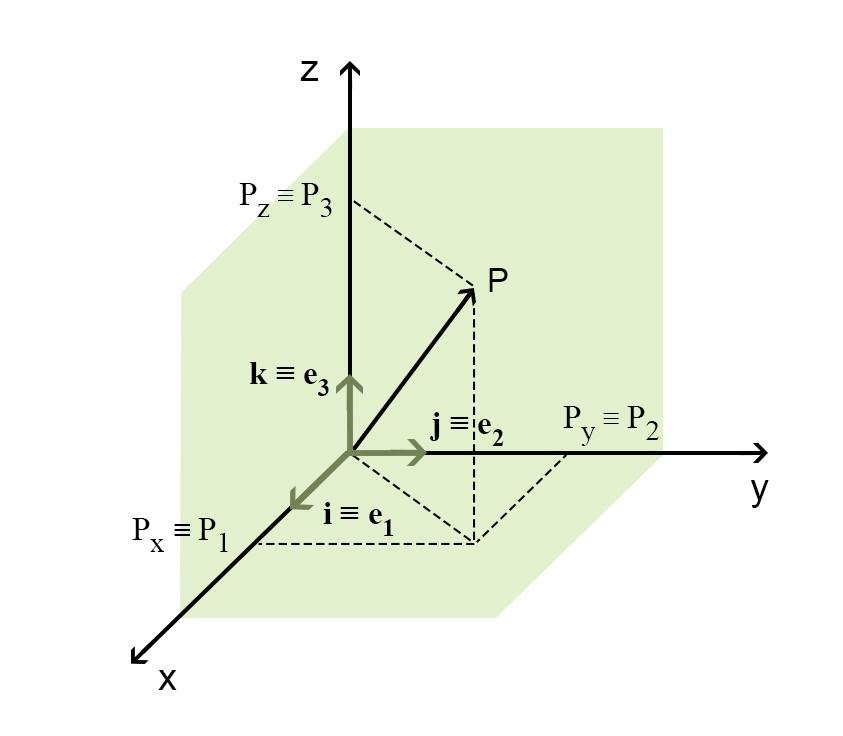
\includegraphics[scale=0.4]{Pictures/Tens_fig10.jpg}
\caption{Vector en el sistema de coordenadas cartesianas.}
\label{Tens_fig10}
\end{center}
\end{figure}



La representación del vector  $\bold{P}$ de la  Ec.(\ref{veccart}) se expresa   con la notación indicial de la forma siguiente  (\cite{chaves}):
\begin{equation}
\bold{P}= P_i \bold{e}_i  \qquad (i=1,2,3)
\end{equation}

%Utilizando notación indicial los ejes del sistema de coordenadas son designados por la letra $x$ con un índice, 
%Por eso $x^i$ no representa un único valor sino $N$ valores si $i=1,2, \cdots, N$.


\subsection{Delta de Kronecker}\index{Delta de Kronecker}
El símbolo \textit{delta de Kronecker}, está definido por

\begin{eqnarray}
\label{Krone}
\delta_{ij} = \left \{
\begin{array}{ll}
1  & \mbox{ si $i=j$}, \\
                     0 & \mbox{ si  $i \neq j$}.
                     \end{array}
                     \right
\end{eqnarray}
\noindent                  
y  coincide con el resultado de hacer el producto escalar entre los vectores de  la base ortonormal $\bold{e}_i$, es decir que $\bold{e}_i   \cdot \bold{e}_j= \delta_{ij}$. Exponiendo esto en forma explícita se tiene:

   \begin{equation}
   \bold{e}_i. \bold{e}_j=
  \left(\begin{array}{ccc} \bold{e}_1 \cdot \bold{e}_1  & \bold{e}_1 \cdot \bold{e}_2  & \bold{e}_1 \cdot \bold{e}_3   \\ \bold{e}_2 \cdot \bold{e}_1 & \bold{e}_2 \cdot \bold{e}_2  & \bold{e}_2 \cdot \bold{e}_3  \\\bold{e}_3 \cdot \bold{e}_1   & \bold{e}_3 \cdot \bold{e}_2 & \bold{e}_3 \cdot \bold{e}_3
\end{array}
 \right) =    \left(\begin{array}{ccc} 1 & 0 & 0 \\0 & 1 & 0  \\0 & 0 & 1
 
\end{array}  \right) = \delta_{ij}
 \label{tensordelta}
\end{equation}

\bigskip


Este símbolo $\delta_{ij}$ es llamado \textit{operador de sustitución }, por la propiedad interesante que mostramos con un ejemplo.

Sea $\mathbf{v}$ un vector de componentes $v_i$, entonces

$$ \delta_{ij}v_i= \delta_{1j}v_1  +  \delta_{2j}v_2  +  \delta_{3j}v_3, $$
\noindent
como $j$ es un índice libre, se tiene:
\bigskip

Si $j=1$, $\delta_{i1}v_i= \delta_{11}v_1  +  \delta_{21}v_2  +  \delta_{31}v_3 =v_1 $

Si $j=2$, $\delta_{i2}v_i= \delta_{12}v_1  +  \delta_{22}v_2  +  \delta_{32}v_3 =v_2 $


Si $j=3$, $\delta_{i3}v_i= \delta_{11}v_1  +  \delta_{21}v_2  +  \delta_{31}v_3 =v_3 $

\noindent
de donde 
$$  \delta_{ij}v_i= v_j$$
\noindent
es decir, por la presencia de $\delta_{ij}$ se reemplaza en la componente $v_i$, el índice $i$ por el $j$. De ahí el nombre de operador de sustitución.

\subsection{Símbolo de Levi-Civita}\index{Símbolo de Levi-Civita}


El símbolo de permutación es llamado también de \textit{Levi-Civita} y está definido por:




\begin{equation}
\label{Levi}
 e_{i_1 i_2  \cdots i_N}=e^{i_1 i_2  \cdots i_N}=
\left\{ \begin{array} {lll} 
                    1 & \mbox{si los índices son distintos y son una permutación par}
\\
                    -1 & \mbox{si los índices son distintos y son una permutación  impar}\\
										 0 & \mbox{en otro caso} \\
                    
                   \end{array}
           \right.
\end{equation}

Es decir depende si  ${i_1 i_2 \cdots i_N}$   es una permutación par o impar de $1, 2, 3, \cdots,  N$.


Este símbolo es utilizado en la definición de determinante de una matriz de $N \times N$:


$$\left  | A \right  | = \sum_{i_1 i_2  \cdots i_N} e_{i_1 i_2  \cdots i_N} \quad a_{1i_1} a_{2i_2}  \cdots a_{Ni_N}$$

El determinante de una matriz $N \times N$ consiste en la suma de todos los productos posibles de $N$ elementos que pertenecen a distintas filas y columnas  multiplicados por $1$ o $-1$ de acuedo a si la permutación de los segundos índices es par o impar
.


\bigskip

En el caso $N=3$ se tiene lo siguiente:

$$e_{ijk}=e^{ijk}= \left[  ~\bold{e}_i~\bold{e}_j~\bold{e}_k   \right] $$



\begin{equation}
\label{Levi}
 e_{ijk}=e^{ijk}=
\left\{ \begin{array} {lll} 
                    1 & \mbox{si $ijk$ es una permutación par de $123$}
\\
                    -1 & \mbox{si $ijk$ es una permutación impar de $123$}\\
										 0 & \mbox{en otro caso} \\
                    
                   \end{array}
           \right.
\end{equation}

\bigskip

Y al calcular el determinante utilizando la definición anterior, se tiene la suma de seis términos, que son  todos los posibles productos de a tres elementos de la matriz

\[
\left  | \begin{array}{ccc}
a_{11}  & a_{12}   & a_{13}  \\
a_{21}  &  a_{22}   &  a_{23}  \\
a_{31}  &  a_{32}   &  a_{33}  
\end{array}
\right|=
\]

\bigskip

$$
=e_{123}~a_{11}a_{22}a_{33}+ e_{231}~a_{12}a_{23}a_{31}+e_{312}~a_{13}a_{21}a_{32}+

+e_{321}~a_{13}a_{22}a_{31}+e_{132}~a_{11}a_{23}a_{32}+e_{213}~a_{12}a_{21}a_{33}
$$


\bigskip

Luego, reemplazando los símbolos de permutación $e_{ijk}$ de acuerdo a (\ref{Levi}), resulta 
\[
\left  | A \right  |= 
a_{11}a_{22}a_{33}+ a_{12}a_{23}a_{31}+a_{13}a_{21}a_{32}-a_{13}a_{22}a_{31}-a_{11}a_{23}a_{32}-a_{12}a_{21}a_{33}
\]


\bigskip

Por otro lado, si se expresa el símbolo de permutación en función de la delta de Kronecker (u operador de sustitución), obtenemos

\begin{equation}
e_{ijk}=e_{lmn}~\delta_{li}\delta_{mj}\delta_{nk}
\end{equation}

\bigskip

\noindent
que es igual al resultado del determinante 


\[
e_{ijk}=\left  | \begin{array}{ccc}
\delta_{1i}  &\delta_{1j}   & \delta_{1k}  \\
\delta_{2i}  &  \delta_{2j}   &  \delta_{2k}  \\
\delta_{3i}  &  \delta_{3j}   &  \delta_{3k}  
\end{array}
\right|
\]


\begin{example}
 \[
e_{321}=\left  | \begin{array}{ccc}
\delta_{13}  &\delta_{12}   & \delta_{11}  \\
\delta_{23}  &  \delta_{22}   &  \delta_{21}  \\
\delta_{33}  &  \delta_{32}   &  \delta_{31}  
\end{array}
\right|= \left  | \begin{array}{ccc}
0  & 0   & 1  \\
0  &  1   &  0  \\
1  & 0   &  0  
\end{array}
\right|= -1
\]   
\end{example}

\section{Operaciones con vectores}
\noindent
\textbf{Producto escalar}\index{Producto escalar}

Dados 
$\bold{u}=~\beta^i~\bold{e}_i$ y  $\bold{v}=~\lambda^j~\bold{e}_j$ con $i,j=1,2, \cdots  n$
el producto escalar es 

\bigskip


$$\bold{u}.\bold{v}=~\beta^1 \lambda^1+ \beta^2 \lambda^2+ \cdots\beta^n\lambda^n = \beta^l\lambda^l $$



\bigskip

%Si suponemos que $\vec{e}^j=\vec{e}_j,j=1,2,\cdots n $, $\vec{v}=~\lambda^j~\vec{e}_j= ~\lambda_j~\vec{e}^j$, podemos  %reescribir el producto escalar $\vec{u}.\vec{v}$ de la forma siguiente:

\bigskip
Esto se obtiene al reemplazar  los vectores  $\vec{u}$ y $\vec{v}$, 
\begin{equation}
\bold{u}.\bold{v}= (~\beta^i~\bold{e}_i).~(\lambda^j~\bold{e}_j)=(~\beta^i \lambda^j) ~(\bold{e}_i.\bold{e}_j)
\label{producto escalar1}
\end{equation}

\bigskip
Usando (\ref{Krone}), como   $\bold{e}_i.\bold{e}_j=\delta_{ij}$, la ecuación ( \ref{producto escalar1}) queda
\begin{equation}
\bold{u}.\bold{v}= (~\beta^i \lambda^j) \delta_{ij}=  ~\beta^i\lambda^i
\label{producto escalar2}
\end{equation}
\bigskip

La  longitud de $\bold{u}$ puede escribirse

\bigskip


$$\left\|\bold{u}\right\|=\sqrt{\beta^i~\beta^i~}$$


La multiplicación de dos matrices $A\in \mathrm{R}^{m\times k }$ y $B\in \mathrm{R}^{k\times n }$ da por resultado una matriz $C\in \mathrm{R}^{m\times n }$. Si indicamos con el supraíndice la fila y con subíndice la columna,  los  elementos de la matriz $C$ son 

\bigskip


$$c^i_j=\sum_{l=1} ^k~a_l^i~b_j^l$$

\bigskip

\noindent
que se simplifica usando el convenio de Einstein a 

$$c^i_j=~a_l^i~b_j^l.$$

\bigskip

\noindent

\begin{remark}
Note que $c^i_j$ tiene dos índices libres. No es un escalar, porque no están todos los índices afectados a sumatorias.
%\hfill$\blacktriangle$
\end{remark}
\newpage
\noindent
\textbf{Producto vectorial}\index{Producto vectorial}

Si $\bold{u_i}= ~\beta_i^j~\bold{e}_j$  son vectores de $\mathrm{R}^{3}$, $i=1,3$, el producto vectorial  de $\bold{u_1}$ y $\bold{u_2}$ da como resultado un vector:
\begin{equation}
\bold{u}_1 \times\bold{u}_2= e_{ijk}~\beta_1^j~\beta_2^k~~\bold{e}_i
\label{producto vectorial}
\end{equation}
donde $e_{ijk}$ es el símbolo de permutación. 
\bigskip
Esa expresión se obtiene a partir de calcular el determinante 

\[
\bold{u}_1 \times\bold{u}_2=\left  | \begin{array}{ccc}
\bold{e}_1  & \bold{e}_2  & \bold{e}_3 \\
\beta_1^1 &  \beta_1^2  &  \beta_1^3 \\
\beta_2^1 &  \beta_2^2  &  \beta_2^3 
\end{array}
\right|=c_1 \bold{e}_1 + c_2 \bold{e}_2  + c_3 \bold{e}_3,
\]

\bigskip
\noindent
donde 
\[
c_1 = \beta_1^2 \beta_2^3 - \beta_2^2  \beta_1^3 \\
c_2 = - \beta_1^1  \beta_2^3  +  \beta_2^1   \beta_1^3  \\
c_3= \beta_1^1  \beta_2^2  - \beta_2^1  \beta_1^2  
\]

Teniendo en cuenta la definición de los símbolos de permutación (\ref{Levi}),  pueden reescribirse 
\[
c_1=e_{123} \beta_1^2 \beta_2^3  + e_{132} \beta_2^2 \beta_1^3 \\
c_2 = e_{231} \beta_1^1  \beta_2^3  + e_{213} \beta_2^1   \beta_1^3  \\
c_3=   e_{312} \beta_1^1  \beta_2^2 +  e_{321} \beta_2^1  \beta_1^2  
\]
luego, en forma reducida, usando la notación de Einstein,


$$c_i=e_{ijk} \beta_1^j \beta_2^k$$  

\noindent
y de ahí se obtiene la expresión (\ref{producto vectorial}).






\bigskip

\begin{example}


Si se desarrolla la expresión $c_i=e_{ijk} A^j B^k $ para $i=1$, se tiene:

\bigskip

\begin{eqnarray*}
c_1&=&e_{1jk} A^j B^k \\
c_1&=& e_{11k} A^1 B^k + e_{12k} A^2 B^k + e_{13k} A^3 B^k \\
c_1&=& e_{111} A^1 B^1 + e_{112} A^1 B^2 + e_{113} A^1 B^3 +  e_{121} A^2 B^1 + e_{122} A^2 B^2 +\\
 &&  + ~ e_{123} A^2 B^3 +    e_{131} A^3 B^1  + e_{132} A^3 B^2  + e_{133} A^3 B^3
\end{eqnarray*}


\bigskip

De acuerdo a la definición de los símbolos de permutación (\ref{Levi}) son nulos los términos con índices repetidos, entonces resulta


\begin{eqnarray*}
c_1=e_{123} A^2 B^3 + e_{132} A^3 B^2= A^2 B^3 - A^3 B^2 
\end{eqnarray*}
\end{example}


\noindent
\textbf{Producto mixto}\index{Producto mixto}

Si $\bold{u}_l=\beta_l^i~\bold{e}_i$  y anotamos como $\left[\bold{u}_1\bold{u}_2\bold{u}_3\right]$ al producto mixto,

 $$\left[\bold{u}_1\bold{u}_2\bold{u}_3\right]= \bold{u}_1.(\bold{u}_2\times\bold{u}_3)$$

\noindent
se tiene que 

\bigskip

$$\left[\bold{u}_1\bold{u}_2\bold{u}_3\right]=\left[ ~\beta_1^i~\bold{e}_i  ~\beta_2^j~\bold{e}_j ~\beta_3^k~\bold{e}_k \right]$$

\bigskip


$$=~\beta_1^i~\beta_2^j~\beta_3^k\left[  ~\bold{e}_i~\bold{e}_j~\bold{e}_k   \right]$$

\bigskip

$$=~\beta_1^i~\beta_2^j~\beta_3^k ~e_{ijk}$$


\bigskip


\noindent
o sea, es el determinante de la matriz de las coordenadas $\beta_j^i $, 

\bigskip

$$\left[\bold{u}_1\bold{u}_2\bold{u}_3\right]=\left|\beta_j^i  \right|$$



\bigskip

\noindent
\textbf{Producto tensorial}\index{Producto tensorial}

El producto tensorial o diádico entre dos vectores $\bold{u}$  y $\bold{v}$ está definido de la forma siguiente:

\begin{equation}
\bold{u} \otimes \bold{v}=  \left[ \begin{array}{c} u_1 \\ u_2
\\  u_3
\end{array}
 \right]  \otimes   \left[ \begin{array}{c} v_1 \\ v_2
\\  v_3
\end{array}
 \right] = \left[ \begin{array}{ccc} u_1 v_1  & u_1 v_2 & u_1 v_3 \\ u_2 v_1  & u_2 v_2 & u_2 v_3
\\  u_3 v_1  & u_3 v_2 & u_3 v_3
\end{array}
 \right]
 \label{ptensvectores}
\end{equation}

\bigskip


Se obtiene una matriz $\bold{A}$, $\bold{A}= \bold{u} \otimes \bold{v} $, donde, por ejemplo, $ u_3 v_2 $ es la  componente de la fila  $3$, y columna $2$. En este caso particular, el producto tensorial es el producto   matricial usual  de los vectores $ \bold{u}$ (de $n \times 1$)  y  $\bold{v}^t$, (de $1 \times n$). 


Una matriz $\bold{A}$ puede escribirse en términos de los productos tensoriales de los vectores de la base $~\bold{e}_1$, $~\bold{e}_2$, y $~\bold{e}_3  $, de la forma siguiente:

\bigskip

\begin{equation}
\bold{A}= \bold{u} \otimes \bold{v}=
u_1 v_1 \left( \begin{array}{ccc} 1  & 0   & 0 \\ 0    & 0 & 0
\\  0 & 0 & 0
\end{array}
 \right)+  u_1 v_2 \left( \begin{array}{ccc} 0  & 1   & 0 \\ 0    & 0 & 0
\\  0 & 0 & 0
\end{array}
 \right)+ 
 
+ u_1 v_3 \left( \begin{array}{ccc} 0  & 0   & 1 \\ 0    & 0 & 0
\\  0 & 0 & 0
\end{array}
 \right)+ \cdots u_3 v_3 \left( \begin{array}{ccc} 0  & 0   & 0 \\ 0    & 0 & 0
\\  0 & 0 & 1
\end{array}
 \right)
\end{equation}




\begin{equation}
\bold{A}= \bold{u} \otimes \bold{v}= u_1v_1 ~ \bold{e}_1 \otimes \bold{e}_1 + u_1v_2  ~\bold{e}_1 \otimes \bold{e}_2 +  \cdots  u_3v_3  ~\bold{e}_3 \otimes \bold{e}_3
\end{equation}

\bigskip

\noindent
que, utilizando el convenio de Einstein, puede  reescribirse
 

\begin{equation}
\bold{A}= \bold{u} \otimes \bold{v}= u_iv_j ~\bold{e}_i \otimes \bold{e}_j 
\end{equation}


\section{ Transformaciones lineales}


%%%%%OJO  ver apunte de tensores de Exactas

Sea $T: V \rightarrow W$ una transformación lineal entre dos espacios vectoriales $V$ y $W$ (ver Definición \ref{TL}).
Sean $B= \left\{\bold{v}_1,\bold{v}_2,\cdots, \bold{v}_N\right\}$ una base  de $V$ y $\bar{B}= \left\{\bold{w}_1,\bold{w}_2,\cdots, \bold{w}_m\right\}$ una base  de $W$. Si aplicamos $T$ a un vector arbitrario $\bold{v}\in V$, 



$$\bold{v}= ~\alpha^j~\bold{v}_j$$



$$T(\bold{v})= T(\alpha^j~\bold{v}_j)= ~\alpha^j~T(\bold{v}_j)$$

\bigskip

Como $T(\bold{v})$ es un elemento de $W$, se puede escribir como combinación lineal de los vectores de la base de $W$, 



$$T(\bold{v})= ~\beta^i~\bold{w}_i$$

\bigskip
Por otro lado, si se aplica $T$ a los vectores de la base de $V$, se obtiene la expresión 

 $$T(\bold{v}_j)=a_j^i~\bold{w}_i$$

\bigskip
\noindent
donde los escalares $a_i^j$ son las coordenadas $T(\bold{v}_j)$ en la base de $W$. 


En la expresión  anterior   el término $a_j^i$  tiene dos índices: $j$ está asociado al espacio  $V$ e $i$ al espacio $W$. $T$ es la matriz de la transformación lineal, en cada columna $j$ están las coordenadas de $T(\bold{v}_j)$ en la base de $W$.


$$T(\bold{v})=~\alpha^j~T(\bold{v}_j)= \alpha^j a_j^i~\bold{w}_i$$



$$T(\bold{v})= ~\beta^i~\bold{w}_i= a_j^i \alpha^j ~\bold{w}_i$$

\bigskip


\noindent
de donde,
 


$$ (~\beta^i~ - a_j^i \alpha^j ) ~\bold{w}_i=\bold{0}$$

\bigskip


\noindent
y por ser los $\bold{w}_i$ linealmente independientes (forman una base de $W$), resulta 



$$ \beta^i~ = a_j^i \alpha^j $$

\bigskip
\noindent
que da la relación entre las coordenadas  de $\bold{v}$ y de $T(\bold{v})$. Corresponde al producto matricial 




%$$A=\left(\begin{array}{cccc} a_{11} & a_{12}&  \cdots & a_{1n} \\a_{21}  & a_{22} & \cdots & a_{2n}
%\\  \cdots & \cdots  &  \cdots  & \cdots \\ a_{n1} & a_{n2} & \cdots & a_{nn}
%\end{array}
% \right)$$

%$$\left[ \begin{array}{c} \beta^1 \\ \beta^2 
%\\  \beta^3\\ \cdots \\ \beta^n
%\end{array}
% \right]  \left[\begin{array}{cccc} a_{1}^1 & a_{2}^1&  \cdots & a_{n}^1 \\a_{1}^2  & a_{2}^2 & \cdots & %a_{n}^2
%\\  \cdots & \cdots  &  \cdots  & \cdots \\ a_{1}^n & a_{2}^n & \cdots & a_{n}^n
%\end{array}
% \right]\left[\begin{array}{c} \alpha^1 \\ \alpha^2   
%\\  \alpha^3  \\ \cdots \\ \alpha^n  
%\end{array}\right] $$


\bigskip

\begin{equation}
    \left(\begin{array}{c} \beta^1 \\ \beta^2 
\\  \beta^3\\ \cdots \\ \beta^n 
\end{array}
 \right)=\left(\begin{array}{cccc} a_{1}^1 & a_{2}^1&  \cdots & a_{n}^1 \\a_{1}^2  & a_{2}^2 & \cdots & a_{n}^2
\\  \cdots & \cdots  &  \cdots  & \cdots \\ a_{1}^n & a_{2}^n & \cdots & a_{n}^n
\end{array}
 \right)\left(\begin{array}{c} \alpha^1 \\ \alpha^2   
\\  \alpha^3  \\ \cdots \\ \alpha^n  
\end{array}\right)
\end{equation}

\bigskip


En los elementos de la matriz el supraíndice $i$ y el subíndice $j$ del elemento $a_j^i$ corresponden a la fila y  a la columna  respectivamente. Es la matriz asociada a la transformación lineal $T$ definida en la Sección \ref{MatrizdeunaTL}).

\bigskip

\begin{example}
\label{ejuiyei}
\noindent
Si la transformación lineal  es la identidad, usamos dos bases distintas, $B=\left\{\bold{e}_1,\bold{e}_2\right\}$ y $B^\prime=\left\{\bold{u}_1,\bold{u}_2,\right\}$, y las coordenadas en cada base son  $\bold{v}= ~\beta^j~\bold{e}_j=~\alpha^j~\bold{u}_j$,   la relación entre las coordenadas es 
$$ \beta^i~ = a_j^i \alpha^j .$$


$$\left(\begin{array}{c} \beta^1 \\ \beta^2 
 \end{array}
 \right)= \left(\begin{array}{cc} a_{1}^1  &a_{2}^1  \\ a_{1}^2\ &  a_{2}^2
\end{array}
 \right)\left(\begin{array}{c} \alpha^1 \\ \alpha^2 
 \end{array}
 \right)$$
 
 \bigskip
 
Estas expresiones se  corresponden con las Ecs.(\ref{ec4}) y (\ref{XPAX}),  donde se vio la relación  entre  las coordenadas del vector $\vec{x}$ en la antigua base  $B$  y en la nueva base $B ^{\prime}$, respectivamente, $x^i$ y $x^{ \prime i}$, con $i=1,2$. En forma matricial, $X=AX^{\prime}$, o 



\begin{equation}
\left\{ \begin{array} {ccl} 
                    x^1&\ =&   a^1_{1}x^{\prime 1}+a^1_{2}x^{\prime 2}    \\
                     x^2 &\ = &a^2_{1}x^{\prime 1}+a^2_{2}x^{\prime 2} 
                   \end{array}
           \right.
\end{equation}



\bigskip

Si $\bold{u}_1=(2,3)$ y $\bold{u}_2=(1,4)$ 
usando lo anterior, para el vector  

\bigskip



$$\left(\begin{array}{c} 7 \\ 7
 \end{array}
 \right)_B=\left(\begin{array}{cc} 2  & 1 \\ 3  &  4
\end{array}
 \right)
\left(\begin{array}{c} 3 \\ 1
 \end{array}
 \right)_{B^\prime}= P_{B,B ^{\prime}}\left(\begin{array}{c} 3 \\ 1
 \end{array}
 \right)_{B^\prime}$$

\bigskip




\bigskip

La relación está dada por la matriz de cambio de base de $B^\prime$ a $B$, $P_{B,B ^{\prime}}$ vista en la  Sección \ref{Cambio de base}.


\bigskip


Por otro lado,  La relación entre los vectores de las bases  $B^\prime$  y $B$ está dada por la matriz transpuesta  (Ver Ec.(\ref{matriz Acb}) en la Sección (\ref{Cambio de base})):



\begin{equation*} \label{rot}
\left\{ \begin{array} {ccl} 
                    \bold{u _1} &\ =&   a_{1}^1\bold{e}_1+a_{1}^2\bold{e}_2 =2\bold{e}_1+3\bold{e}_2   \\
                     \bold{u _2 } &\ = &a_{2}^1\bold{e}_1+ a_{2}^2\bold{e}_2 =1\bold{e}_1+4\bold{e}_2  \\
										\end{array}
           \right.
\end{equation*}

\bigskip


Usando el convenio, la relación entre los vectores de las bases tiene la expresión


 $$ \bold{u}_j~ = a_j^l \bold{e}_l$$

\end{example}

%\subsection{Transformaciones de coordenadas ortogonales}


%\bigskip

\noindent
 %mientras que la  relación entre  las coordenadas de un mismo vector en las bases $B$ y $B^\prime$  (ver %Sección(\ref{RELCOORD}), Ec.(\ref{ec4})), está dada por:






\section{Definición de tensor}


El concepto de \emph{tensor} tiene su origen en la evolución de la geometría diferencial de Gauss, Riemann y Christoffel. La necesidad del cálculo tensorial, como rama sistemática de la matemática, se debe a Ricci y a su discípulo Levi-Civita, que publicaron en colaboración el primer trabajo sobre esta materia: \emph{Métodos del cálculo diferencial absoluto y sus aplicaciones}, en Mathematische Annalen, vol. 54 (1901).



El objeto principal del cálculo tensorial es la investigación de las relaciones que permanecen invariantes cuando se cambia de un sistema de coordenadas a otro. Las leyes de la física no pueden depender del sistema de referencia que elija el físico con fines descriptivos. Por eso es, estéticamente deseable y muchas veces conveniente, utilizar el cálculo tensorial como fundamento matemático en que se puedan formular tales leyes. Einstein, en particular, lo consideró un excelente instrumento para la presentación de su teoría general de la relatividad. El cálculo tensorial alcanzó gran importancia y es hoy en día inapreciable en sus aplicaciones en la mayoría de las ramas de la física teórica; es también indispensable en  geometría diferencial.




\begin{figure}[hbtp]
%\centering
\begin{center}
%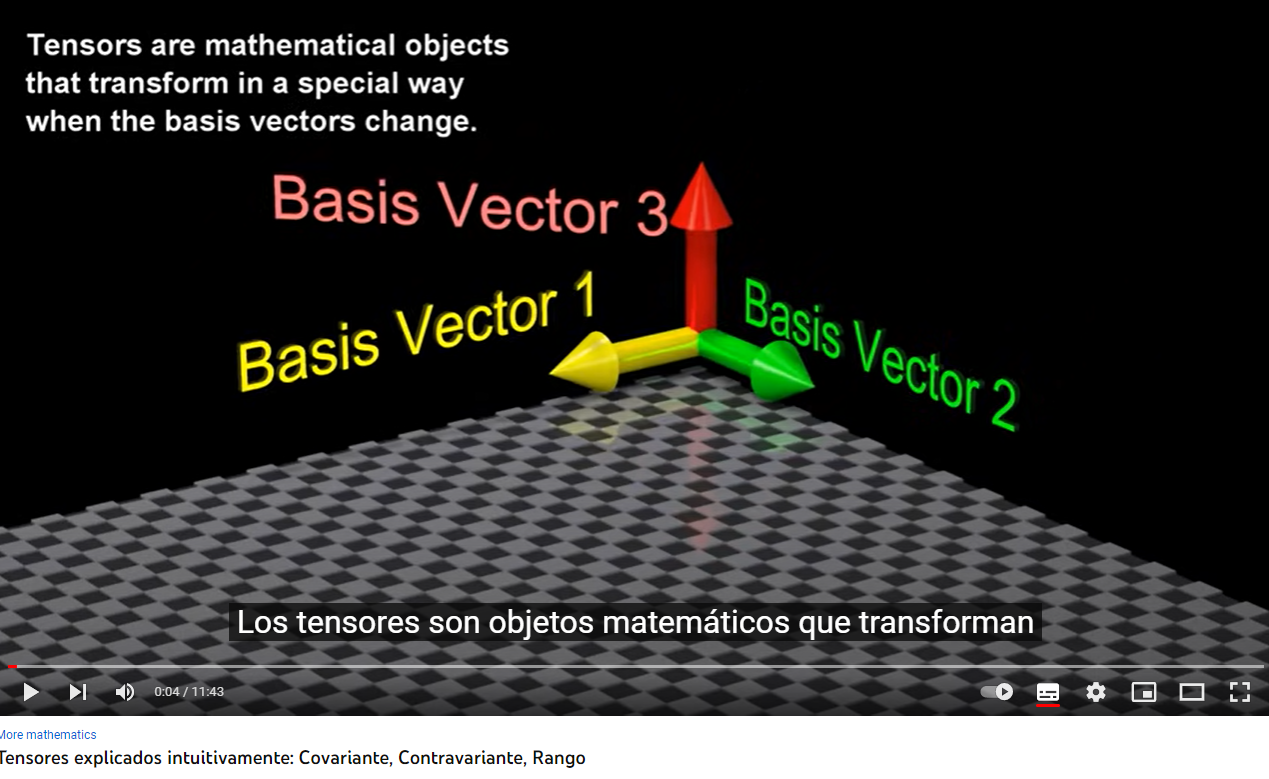
\includegraphics[scale=0.35]{Pictures/VIDEO_tensores.png}
%\caption{}
\end{center}
\end{figure}

\bigskip


%Los tensores se definen en función de sus propiedades de transformación ante un cambio de coordenadas:
\subsection{Cambio de coordenadas}




Si se considera un espacio vectorial $V$ de dimensión $N$ con el sistema de coordenadas $  x^1, x^{2}, x^{3},\cdots,x^{n}$, las $N$ ecuaciones 




\begin{equation}
x^{\prime i} = x^{\prime i}( x^1, x^{2}, x^{3},\cdots,x^{n} )= \varphi ^i( x^1, x^{2}, x^{3},\cdots,x^{n} ), \qquad i=1, \cdots N
\label{cambiocoord}
\end{equation}

\bigskip
\noindent
donde $  \varphi ^i$  son funciones continuas y diferenciables de las coordenadas  definen un nuevo sistema de coordenadas  $  x^{\prime 1}, x^{\prime 2}, \cdots, x^{\prime N}$.

\bigskip

La condición necesaria y suficiente para que las Ec.(\ref{cambiocoord}) definan una transformación de coordenadas 
es que el Jacobiano formado por las derivadas parciales $  \frac{\partial  x^{\prime i}}{\partial   x^{j}}$ no se anule.
En ese caso se pueden resolver para las $  x^i$  como funciones de $  x^{\prime i}$ y se obtiene, 
\begin{equation}
x^{i} = \psi ^i( x^{\prime 1}, x^{\prime 2}, \cdots, x^{\prime N} ), \qquad i=1, \cdots N
\label{cambiocoord2}
\end{equation}


\bigskip

\begin{example}
\label{ejrelcont2}
 En el caso particular de un cambio de base en $\mathbb{R}^3$   la relación entre las coordenadas está dada por el sistema lineal (\ref{ec4}) para $n=3$


\begin{equation}
\left\{ \begin{array} {ccl} 
                    x^1&\ =&   a^1_{1}x^{\prime 1}+a^1_{2}x^{\prime 2}+a^1_{3}x^{\prime 3}    \\
                     x^2 &\ = &a^2_{1}x^{\prime 1}+a^2_{2}x^{\prime 2}+a^2_{3}x^{\prime 3} \\
                    x^3 &\ =&a^3_{1}x^{\prime 1}+a^3_{2}x^{\prime 2}+a^3_{3}x^{\prime 3}
                   \end{array}
           \right.
\end{equation}

Corresponde a  relaciones como  las de la Ec.(\ref{cambiocoord2}). El determinante de la matriz Jacobiana (cuyos elementos son $  \frac{\partial  x^{i}}{\partial   x^{\prime}_j}= a^i_{j}$) no se anula, porque   la matriz de cambio de base $A$ tiene inversa. Con su matriz inversa  pueden escribirse  las ecuaciones    (\ref{cambiocoord}) y así tener   las coordenadas $x^{\prime i}$ como funciones de las  $x^i$.
\end{example}
\subsection{Tensores de orden $0$, $1$ y $2$}
\label{T012}
Es importante tener presente la expresión  (\ref{XPAX})  de la relación ya vista  entre las coordenadas $x^{\prime i}$ y $x^{i}$  ante un cambio de base. Porque los tensores se definen en función de sus propiedades de transformación ante un cambio de coordenadas  (\cite{spain}).:
\begin{equation}
\label{Cambiocoord}
x^{i} \rightarrow x^{\prime i}  \qquad i=1,\cdots,N
\end{equation}
dado por las relaciones de las Ecs.(\ref{cambiocoord}) y (\ref{cambiocoord2}).

\bigskip

Se tiene lo siguiente:

\bigskip

\begin{itemize}
\item
\textbf{Tensor de orden cero o escalar} es una cantidad $\phi$ que permanece invariante al cambiar al sistema primado,

$$\phi^{\prime}=\phi$$

\textcolor{blue}{Ejemplos}
La masa, la energía, la temperatura.

\bigskip

 \item
\textbf{Tensor de orden uno o vector} son $N$ cantidades



\bigskip
\begin{itemize}
\item  
\textbf{Vectores contravariantes}

Las funciones $  v^{j}$   de las $N$ coordenadas $  x^{i}$  se dice que son las componentes de un \textit{vector contravariante} si se transforman según la ecuación:


\begin{equation}
v^{\prime i} = \sum^{n}_{i=1} \frac{\partial  x^{\prime i}}{\partial   x^{j}} \quad v^{j} = \frac{\partial  x^{\prime i}}{\partial   x^{j}} \quad  v^{j} \qquad i=1,\cdots,n 
\label{contravariante}
\end{equation}
en un cambio de coordenadas de $ x^{i}$  a $ x^{\prime i}$.
  
\bigskip

\textcolor{blue}{Ejemplo}  
Los diferenciales $d x^{\prime i} $,  
\[d x^{\prime i}= \frac{\partial  x^{\prime i}}{\partial   x^{j}} \quad  dx^{j}   \]
forman las componentes de un vector contravariante, ya que 
se transforman de la misma forma que la expresión (\ref{contravariante}).
\bigskip 

\item 

\textbf{Vectores covariantes}

Las funciones $  v_{j}$   de las $N$ coordenadas $  x^{i}$  se dice que son las componentes de un \textit{vector covariante} si se transforman según la ecuación:


\begin{equation}
v_i^{\prime}=\frac{\partial  x^{j}}{\partial   x^{\prime i}} \quad  v_{j}
\label{covariante}
\end{equation}
en un cambio de coordendas de $ x^{i}$  a $ x^{\prime i}$.
\bigskip
Ejemplo.
El vector gradiente de una función $f$
\begin{equation}
\frac{\partial  f }{\partial   x^{\prime i}}=\frac{\partial  f}{\partial   x^{j}} \frac{\partial  x^{j}}{\partial   x^{\prime i}}= \frac{\partial  x^{j}}{\partial   x^{\prime i}}\frac{\partial  f}{\partial   x^{j}}
\end{equation}
De acuerdo a la Ec.(\ref{covariante}) las magnitudes $  \frac{\partial  f}{\partial   x^{j}}$  son las componentes de un vector covariante (en esa expresión el índice $j$ es considerado un subíndice).



\bigskip 

\textcolor{blue}{Ejemplos} de tensores de orden $1$: $\bold r$, vector posición y  $\bold v$ vector velocidad.

\bigskip

\end{itemize}
\item
\textbf{Tensor de segundo orden: son $N^{2}$ cantidades}:

\bigskip

\begin{itemize}
\item 

$t^{ij}$ ($i,j=1, \cdots,N$) son las componentes de un tensor  dos veces contravariante 
si se transforman según 

\bigskip


\begin{equation}
t^{\prime ij}= \frac{\partial  x^{\prime i}}{\partial   x^{l}}  \frac{\partial  x^{\prime j}}{\partial   x^{m}} \quad  t^{lm}
\end{equation}

\bigskip

\item 

$t_{ij}$ ($i,j=1, \cdots,N$) son las componentes de un tensor  dos veces covariante 
si se transforman según 
\begin{equation}
t^{\prime}_{ij}= \frac{\partial  x^{l}}{\partial   x^{\prime i}}  \frac{\partial  x^{m}}{\partial   x^{\prime j}} \quad  t_{lm}
\end{equation}

\bigskip

\item


$t^{i}_{j}$ ($i,j=1, \cdots,N$) son las componentes de un tensor  una vez contravariante   y otra covariante si se transforman según

\begin{equation}
t^{\prime i}_{j}= \frac{\partial  x^{\prime i}}{\partial   x^{l}}  \frac{\partial  x^{m}}{\partial   x^{\prime j}} \quad  t^{l}_{m}
\end{equation}

\bigskip

o, 
\begin{equation}
t^{\prime j}_{i}= \frac{\partial  x^{l}}{\partial   x^{\prime i}}  \frac{\partial  x^{\prime j}}{\partial   x^{m}} \quad  t_{l}^{m}
\end{equation}





\end{itemize}
\end{itemize}

\bigskip


Los tensores de segundo orden están asociados  a matrices:

\bigskip

$$t_{ij}=\left(\begin{array}{ccccc} t_{11} & t_{12}& & \cdots& t_{15}\\ t_{21}   &  t_{22}  &  &  & \\ t_{31}  &  &  &  &  \\ t_{41} &  &  &  &  \\ t_{51}  &  & \cdots &  & t_{55} 
\end{array}
 \right),  \qquad \qquad t^{i}_{j}=\left(\begin{array}{ccccc} t^{1}_{1} & t^{1}_{2}& & \cdots& t^{1}_{5}\\ t^{2}_{1}   &  t^{2}_{2}  &  &  & \\ t^{3}_{1}  &  &  &  &  \\ t^{4}_{1} &  &  &  &  \\ t^{5}_{1}  &  & \cdots &  & t^{5}_{5}
\end{array}
 \right) $$

 
\bigskip 
 

Como ejemplo, en  (\ref{ptensvectores}) se obtuvo un tensor de segundo orden $\bold{A}$, a partir del producto tensorial de dos vectores.  
 
 
 

% VER El producto de componentes de tensores de rango $n$ por rango $m$ da un tensor de rango $n+m$. Por ejemplo
%\begin{itemize}
%\item  
%$$v^{i}w^{j}=T^{ij}$$
%\item  $$v_{i}w^{j}=T_i^{j}$$%

%\end{itemize}

\subsection{Suma. Contracción de índices.}\index{Contracción de índices}
La suma de tensores de igual orden es un tensor del mismo orden, y el producto de un escalar por un tensor de orden $q$ da un tensor de orden $q$.
El producto de componentes de un tensor por las componentes de otro da las componentes de un tensor de orden suma de los órdenes originales.


\bigskip 

\begin{example}
    

Si $u_i$ son las componentes de un vector y $t_{ij}$ son las componentes de un tensor de orden $2$,
$$u_it_{lm}$$ 
son las componentes de un tensor de orden $3$, ya que tiene $3$ índices libres.
\end{example}





Una operación importante entre tensores es la llamada \textit{contracción de índices}. Es la operación de multiplicar 2 tensores de orden $n$ y $m$ y hacer la suma sobre uno de los índices (de $1$ a $N$). Se obtiene un tensor de orden $n+m-2$.

También  puede realizarse incluso sobre el mismo tensor:
$$T^{i}_{i}$$
obteniéndose un nuevo tensor de rango $n-2$  (es un escalar o tensor de orden 0 para $n=2$, como se vió en el ejemplo de la traza  en la Sección \ref{Convenio}).


\begin{example}
Si se tiene un tensor de orden $3$, de componentes $t_{ijk}$, contrayendo el segundo y tercer índice se obtiene un tensor de orden $1$:

$$  v_i=t_{ijj} $$
\end{example}

    
\begin{example}
Dados $2$ tensores de orden $2$, en este caso $n=m=2$, al sumar sobre el índice $j$:
%(uno contravariante y el otro covariante) 


\begin{equation}
T^{ij}H_{jm}=T^{i1}H_{1m}+T^{i2}H_{2m}+\cdots = S^{i}_{m}
\end{equation}

\bigskip 

\noindent
se tiene  como resultado un tensor de rango $n+m-2=2+2-2=2$. 

\end{example}



\begin{remark}
    

El producto escalar de $2$ vectores ($n=m=1$) es un caso particular  y el resultado es un escalar o tensor de orden $0$. 
\end{remark}


\bigskip 
\begin{example}
Aparece con frecuencia la contracción de uno de los índices  de un tensor de orden $2$ con el índice de un vector (corresponde al producto escalar del tensor por el vector) y da como resultado un vector:
$$v_i=t_{ij}u_j$$ 
\end{example}
  %Para demostrar que efectivamente se obtiene un vector se analiza cómo se transforma ante cambios de %coordenadas.
  
%\begin{eqnarray}
%v^{'}_i&=& t^{'}_{ij}  u^{'}_j = a_{ik}a_{jl}t_{kl} a_{jm}u_m\\
%&=& a_{ik}(a_{jl} a_{jm}) t_{kl} u_m   \\
%&=& a_{ik} \delta_{lm}t_{kl} u_m = a_{ik} t_{kl} u_l = a_{ik} v_k
%\end{eqnarray}
%que es la ley de transformación de las componentes de un vector (considerando una transformación %ortogonal).



Un tensor es \textit{simétrico} respecto a dos de sus índices si al permutarlos se obtiene el mismo valor, por ejemplo 


$$t_{ij}= t_{ji}$$


o 

$$ h_{ijkl}= h_{ilkj} $$

(respecto al segundo y cuarto índice).
Será \textit{antisimétrico} si cambia de signo:  

$$t_{ij}= - t_{ji}$$


o 

$$ h_{ijkl}= - h_{ilkj} $$


Se dice que es \textit{totalmente simétrico} o \textit{totalmente antisimétrico} cuando se cumple lo anterior respecto de cualquier par de índices.
\bigskip


\begin{remark}
Se llama \textit{tensor isotrópico} a un tensor cuyas componentes son las mismas en cualquier sistema de coordenadas. Todo  escalar es un tensor isotrópico pero no hay vector no nulo que sea isotrópico.
Se puede mostrar que todo tensor isotrópico de orden $2$  es un escalar por la delta de Kronecker $\delta_{ij}$ y todo tensor isotrópico de orden $3$ es un escalar por los símbolos de Levi-Civita.
%\hfill$\blacktriangle$
\end{remark}




%\subsection{Transformaciones ortogonales}

%Pasan de sistemas de coordenadas cartesianas ortogonales a otro similar. Son lineales; además de teener en cuenta la ortogonalidad de %ambos sistemas de jes, se llega a que la matriz inversa de la matriz $A$ debe seer igual a su traspuesta.

%$$A^{-1}=A^{T}$$ 
%$$A.A^{T}=I$$

%o sea, 


%\begin{equation}
%a^{i}_{j}(a^{T})^{j}_{l}=\delta^{i}_{l}
%\end{equation}

%($ \sum_{j} a^{i}_{j}a^{l}_{j}=\delta^{il}$)
\index{Levi-Civita, Tullio}
\begin{parchment}[Tullio Levi-Civita (1873 - 1941)]{ Fue un matemático italiano, famoso por su trabajo sobre cálculo tensorial, pero que también hizo contribuciones significativas en otras áreas de las matemáticas. Era discípulo de Gregorio Ricci-Curbastro, el inventor (algunos dicen co-inventor con Levi-Civita) del cálculo tensorial. Su trabajo incluye artículos fundamentales en matemáticas puras y aplicadas, la mecánica celeste (notable en el problema de los tres cuerpos) e hidrodinámica.
Levi-Civita personalmente ayudó a Albert Einstein a aprender el cálculo tensorial, en el cual Einstein basaría su relatividad general, y que había luchado por dominar. Su libro de texto en cálculo tensorial El Cálculo Diferencial Absoluto (originalmente un conjunto de notas de la conferencia en italiano de coautoría con Ricci-Curbastro) sigue siendo uno de los textos estándares más de un siglo después de su primera publicación, con varias traducciones disponibles. \cite{levi}}
\end{parchment}











\subsection{Transformaciones ortogonales }

Vimos que si se aplica una transformación lineal la relación entre las coordenadas en distintas bases está dada por la expresión, (ver Sección \ref{Cambio de base} y el Ejemplo \ref{ejuiyei})
\begin{equation}
\label{TL0}
x^{j} =  a^{j}_{i}x^{\prime i}
\end{equation}
donde $a^{j}_{i}$ son los elementos de la matriz cambio de base. 

\bigskip


 A partir de la Ec.(\ref{TL0}), si $B=A^{-1}$ se tiene que 
\begin{equation}
\label{xpxnueva}
 x^{\prime i}= b^i_{j}x^j 
\end{equation}
\noindent
entonces las coordenadas se transforman mediante una ley contravariante .
\bigskip
%Se verá la relación entre la matriz de  cambio de base y las expresiones (\ref{contravariante}) y %(\ref{covariante}).

En la Ec.(\ref{contravariante}),   las cantidades $\frac{\partial  x^{'i}}{\partial   x^{j}}$ son, 

\begin{equation}
\frac{\partial  x^{\prime i}}{\partial   x^{j}} = b^{i}_{j}
\end{equation}

\bigskip
así que, se tiene 
\begin{equation}
x^{\prime i} = \frac{\partial  x^{\prime i}}{\partial   x^{j}} x^{j} = b^{i}_{j}   ~  x^{j} \qquad i=1,\cdots,n 
\label{contrax}
\end{equation}
\noindent
entonces, las coordenadas se transforman mediante una ley contravariante .

%Luego, en la expresión de la Ec.(\ref{covariante}), corresponde 

%\begin{equation}
%\frac{\partial  x^{j}}{\partial   x^{\prime i}} = a^{j}_{i}
%\end{equation}







De la misma manera, un tensor de segundo rango dos veces contravariante se transforma de la forma siguiente:
\begin{equation}
\label{Tpij}
T^{\prime ij} = a^{i}_{l}a^{j}_{m}T^{lm}
\end{equation}

%De la expresión Ec.(\ref{TL0}) se ve que para transformaciones lineales los vectores contravariantes se %transforman como las coordenadas.



Las transformaciones ortogonales son un caso particular de transformaciones lineales, son aquellas  que  transforman un sistema de coordenadas cartesianas ortogonales en otro similar también ortogonal y son tales que la inversa de la matriz que la representa es igual a su transpuesta. Corresponden a rotaciones o reflexiones  (ver  matriz ortogonal Definición  \ref{Matriz ortogonal}, y el Ejemplo \ref{mrotacion} de la Sección \ref{MatrizdeunaTL}).
Es decir 

$$A^{-1}= A^t$$

o bien $$  a^i_{~j} (a^t)^j_{~l}  = \delta^i_{ ~l} $$


o 
$$  a^i_{~j} a^l_{~j} = \delta^{ il} $$

\begin{example}
 Las ecuaciones que corresponden a una rotación de un ángulo $\phi$ alredor del eje $z$  son (ver Ec.(\ref{cambiocoord}) y el Ejemplo \ref{ejrelcont2}).
\begin{eqnarray}
x^{\prime 1}&=&cos(\phi) x^1+ sen(\phi) x^2 \\
x^{\prime 2}&=&-sen(\phi) x^1+ cos(\phi) x^2 \\
x^{\prime 3}&=&x^3
\end{eqnarray}

Es una transformación ortogonal ya que la inversa de la matriz que la representa es igual a su transpuesta, o sea $A^t. A=I$ (ver Sección \ref{Transf.Ortogonales}).



%Como $ x^{'i}= a_{ij}x^j $

%$e_i=a_{jk} x^k \bold{e}^{'}_j $

%Para un punto cuyas coordenadas en el sistema sin primar sean $x^j= \delta_{ij}$ se tendrá un vector %posición $ \vec{r}$ que se puede expresar en los dos sistemas de coordenadas:
%$  \vec{r}=\bold{e}_i= x^{'j}  \bold{e}^{'}_j$. Reemplazando en la expresión anterior, se tiene

%$e_i=a_{jk} \delta_{ik} \bold{e}^{'}_j =a_{ji} \bold{e}^{'}_j $.


%En el caso de transformaciones ortogonales se tiene que los versores en ambos sistemas son ortogonales, %o sea,  se verifica 

%$ \bold{e}_i \cdot \bold{e}_j = \delta_{ij} $

%$ \bold{e}^{'}_i \cdot \bold{e}^{'}_j = \delta_{ij} $.

%Luego


%$  \delta_{ij}= \bold{e}_i \cdot \bold{e}_j= a_{ki}a_{lj} \bold{e}^{'}_k \cdot \bold{e}^{'}_l   $

%$  \delta_{ij}= a_{ki}a_{lj} \delta_{kl}= a_{ki}a_{kj}   $.

%Esta última expresión  de la derecha es el producto de $A^t. A$. Resulta, entonces que $A^t. A=I$. 

Como se vió en la Proposición \ref{det1ortog}, si el determinante  es $1$ corresponde a una rotación y si es $-1$ corresponde a una reflexión (o a una composición de una simetría y una rotación).
\end{example}

\bigskip
\begin{example}
\textbf{Una transformación no ortogonal}

Las transformaciones de Lorentz relacionan las coordenadas en dos sistemas de referencia inerciales
$( x^0, x^1, x^2, x^3) $  y $  (x^{\prime 0}, x^{\prime 1}, x^{\prime 2}, x^{\prime 3})$.

Son las que dejan invariante 
$ s^2=  (x^{\prime 0})^2- (x^{\prime 1})^2 - ( x^{\prime 2})^2- (x^{\prime 3}))^2$.
\noindent
y su relación en forma matricial es la siguiente:



$$\left( \begin{array}{c} x^{\prime 0} \\ x^{\prime 1} 
\\  x^{\prime 2}\\ x^{\prime 3} 
\end{array}
 \right)  \left(\begin{array}{cccc} \gamma & -\beta \gamma &  0 & 0 \\-\beta \gamma  & \gamma & 0  & 0
\\  0 & 0  &  1 & 0 \\ 0 & 0 & 0 & 1
\end{array}
 \right)\left(\begin{array}{c} x^{0} \\ x^{1} 
\\  x^{2}\\ x^{3} 
\end{array}\right) $$
 
\bigskip
 
donde $\gamma = \frac{1}{\sqrt{1-\frac{V^2}{c^2}}}$ es el factor de Lorentz 
y $\beta= \frac{V}{c}$ es la velocidad relativa respecto de la luz ($V$ es la velocidad del movimiento uniforme y $c$ es la velocidad de la luz en el vacío).

La matriz inversa  se obtiene cambiando $\beta$ por $-\beta$, y por lo tanto se tiene que $A^{-1} \neq A^t$. No es una transformación ortogonal.
\end{example}

%\section{Sistema de coordenadas cartesianas}





\section{Tensores cartesianos}
Como se  mencionó  en la Sección \ref{T012} los tensores están definidos por las propiedades de transformación de sus componentes ante cambios de coordenadas. 

Se llaman \textit{tensores cartesianos} a los tensores que están definidos por sus propiedades ante transformaciones entre sistemas de coordenadas cartesianos ortogonales ( ver \cite{santalo}). 
Esto los diferencia de los tensores en general, en los que se consideran transformaciones más generales de coordenadas.  
En los tensores cartesianos no es necesario  diferenciar entre componentes covariantes y contravariantes ya que se transforman igual:  

En este caso, la Ec.(\ref{TL0}) puede escribirse 
\begin{equation}
\label{TL0C}
x^{'}_i =  a_{ij}x_{j}
\end{equation}
donde $a_{ij}$ son los elementos de la matriz cambio de base. 

Los tensores de orden $1$ se transforman con la ley 


\begin{equation}
v^{'}_i= a_{ij}v_j
\end{equation}

Ya que si se utilizan las  relaciones (\ref{contravariante}) y (\ref{covariante}), como $A^t.A=I$, se obtiene:

\begin{equation}
v^{'i}= a^{i}_{j}v^{j}
\end{equation}

\begin{equation}
v^{'}_{i}= (a^{-1})^{j}_{i}v_{j}=(a^{T})^{j}_{i}v_{j}=a^{i}_{j}v_{j}
\end{equation}
 Análogamente, en el caso de tensores de orden $2$, la expresión de la Ec.(\ref{Tpij}) se reescribe 
 
\begin{equation}
\label{Tpijc}
t^{'}_{ij} = a_{il}a_{jm}t_{lm}
\end{equation}

Si se asocian las componentes $t_{ij}$ a una matriz $T$, esta ley de transformación de (\ref{Tpijc}) corresponde a la transformación 
\begin{equation}
T^{'} = ATA^t
\end{equation}


%En general, un tensor de orden $q$ son $N^q$ cantidades $t_{ i_1, i_2, \cdots i_q}$ que ante el cambio de coordenadas %se transforman con la ley

%\begin{equation}
%\label{Tpijcq}
%t^{'}_{ i_1, i_2, \cdots, i_q} = a_{i_1 j_1} a_{i_2 j_2} \cdots a_{i_q j_q}  t_{ j_1, j_2, \cdots, j_q}
%\end{equation}



\begin{figure}[ht]
\label{Tens_fig11}
%\centering
\begin{center}
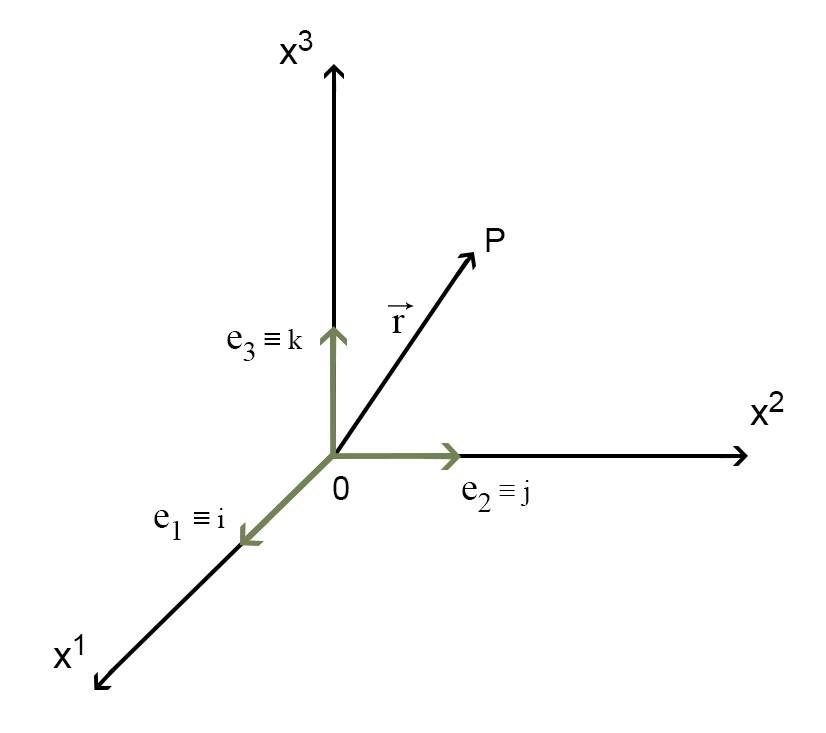
\includegraphics[scale=0.4]{Pictures/Tens_fig11.jpg}
\caption{Bases en coordenadas cartesianas.}
\end{center}
\end{figure}

Ejemplos de tensores cartesianos: el vector posición $\bold{r}$, el vector velocidad $\bold{v}$, el  tensor de inercia $I_{ij}$,  y el tensor de tensiones  $\bold{\tau}_{ij} $.

\section{Sistema de coordenadas curvilíneas}
Las transformaciones de coordenadas se presentaron en las Ecs.
(\ref{cambiocoord}) y  (\ref{cambiocoord2}) de la Sección \ref{Cambiocoord}. Consideremos ahora, en particular, una región del espacio de tres dimensiones referida a un sistema de ejes cartesianos ortogonales,  caracterizados con  supraíndices $x^{1}$, $x^{2}$, y $x^{3}$.

Sean, además
 
\begin{equation}
\overline x^{i} = \overline x^{i}( x^1, x^{2}, x^{3}),  \qquad i=1,2,3
\label{transf1}
\end{equation}



\noindent
funciones continuas con derivadas parciales primeras continuas y tal que el 
jacobiano formado por las derivadas parciales $\frac{\partial \overline x^i}{\partial  x^j}$  no se anule.

\bigskip


Entonces las ecuaciones anteriores pueden resolverse en las $x^{i} $, esto es


\begin{equation}
x^{j} = x^{j}(\overline x^1,\overline x^{2}, \overline x^{3}),  \qquad j=1,2,3
\label{transf2}
\end{equation}

\bigskip

Las variables $\overline x^{i}$ introducidas  son tales que a cada punto $P$   le corresponde una única terna de valores de ellas y recíprocamente: las denominamos coordenadas \textit{curvilíneas} de $P$.


Uno de los  sistemas de  coordenadas curvilíneas más usados en el espacio son las coordenadas cilíndricas $(r,\varphi,z)$, donde,
$\overline x^{1}=r$, $\overline x^{2}=\varphi$ y $\overline x^{3}=z$.
y tales que las  relaciones con las cartesianas $  ( x^1, x^{2}, x^{3})$ son 

$$r= \sqrt{  (x^1)^2  +  (x^2)^2} $$
$$ \varphi= arctan( \frac{x^2}{x^1})$$
$$z=x^3$$

Es decir que  la Ec.(\ref{transf1}) expresa la transformación  entre coordenadas cartesianas y coordenadas cilíndricas. En otro caso puede expresar la transformación  entre coordenadas cartesianas y coordenadas esféricas, otro sistema que  también es usado con frecuencia.

Es importante notar que cuando se pasa de un sistema de coordenadas cartesianas a otras cartesianas, la transformación es lineal, y la relación entre las coordenadas de un mismo punto en los dos sistemas diferentes se obtiene  multiplicando por una matriz. 


\bigskip


Igualando a una constante la Ec.(\ref{transf1})

\bigskip

$\overline x^{i} = \overline x^{i}( x^1, x^{2}, x^{3})= C_i =$ constante, 

\bigskip

\noindent
obtenemos la ecuación de una superficie para cada valor de la constante: es decir que la última ecuación  representa para cada $i=1,2,3$ tres familias de superficies, que se denominana \textit{superficies coordenadas} y la condición que el jacobiano no se anule, significa geométricamente  que tres de ellas (una de cada familia) se intersecan en uno y sólo un punto $P$.

\bigskip

La intersección de las tres superficies   que pasan por $P$ determinan tres líneas, a lo largo de las cuales sólo una coordenada $\overline x^i$ es variable: se denominan líneas coordenadas.
%Continuamos  utilizando  la convención de Einstein, es decir, cuando en una expresión   se repite un índice en un %término, se entiende que implica una suma con respecto a aquel índice, desde $1,2, \cdots, N$  (en este caso $N=3$). Y %usamos también la delta de Kronecker, definida así:

\bigskip
%$$\delta_{ij}=\delta_{i}^{j}= 1 \qquad i=j$$
%$$\delta_{ij}=\delta_{i}^{j}= 0  \qquad i\neq j $$








%Los versores  $\bold{e}_{i}$,  $\overline {\bold{e}}_{i}$ se relacionan mediante:


%\begin{eqnarray}\label{ec_7}
%\bold{e}_{i}= \frac {\partial  \overline x^{j}}{\partial  x^{i}}\overline {\bold{e}}_{j}  \qquad
%\overline {\bold{e}}_{i} = \frac {\partial  x^{j}}{\partial \overline x^{i}}\bold{e}_{j},
%\end{eqnarray}

\bigskip


%($ x^{j}$ y  $\overline x^{j}$ coordenadas curvilíneas).


\bigskip



%\subsection{Elemento de arco}


\subsection{Tensor fundamental (o Tensor Métrico).}\index{Tensor Métrico}

Supongamos se requiere calcular la longitud de un vector $\bold{v}$ dado de $R^3$, por ejemplo $\bold{v}=(7,4,-1)$. Entonces:

\begin{itemize}
    \item 
  Al estar dadas   sus coordenadas  en la base canónica  $B= \left\{\bold{e}_1,\bold{e}_2, \bold{e}_3\right\}$, (sino se hubiera anotado  $\bold{v}=(7,4,-1)_{\overline B}$)  para hallar la longitud  del vector $\bold{v}=(7,4,-1)$ se calcula $\| \bold v\|^2 = (7)^2+(4)^2+(-1)^2= 49+16+1=66$. Se obtiene que su longitud es  $\| \bold v\|=\sqrt{66}.$
     \item
     
Si se tienen las coordenadas de $\bold{v}$ en la base $B^{\prime} =\left\{(1,1,0), (4,2,1),(2,1,-2)\right\}$,  $\bold{v}=(1,1,1)_{B}$, se deben transformar sus coordenadas a la base canónica para calcular la longitud.
\end{itemize}



\bigskip 
 
 
 Es deseable, entonces,  una definición de longitud de un vector invariante ante un cambio de base. Con  el llamado \textit{tensor métrico} se redefine la longitud de un vector según la expresión: 
 
   \begin{equation}
\left(\begin{array}{ccc} x & y & z 
\end{array}
 \right) \left(\begin{array}{ccc} \overline {\bold{e}}_1 \cdot \overline {\bold{e}}_1  & \overline {\bold{e}}_1 \cdot \overline {\bold{e}}_2  & \overline {\bold{e}}_1 \cdot \overline {\bold{e}}_3   \\ \overline {\bold{e}}_2 \cdot \overline {\bold{e}}_1 & \overline {\bold{e}}_2 \cdot \overline {\bold{e}}_2  & \overline {\bold{e}}_2 \cdot \overline {\bold{e}}_3  \\\overline {\bold{e}}_3 \cdot \overline {\bold{e}}_1   & \overline {\bold{e}}_3 \cdot \overline {\bold{e}}_2 & \overline {\bold{e}}_3 \cdot \overline {\bold{e}}_3
\end{array}
 \right)  \left(\begin{array}{c} x \\y  \\z
\end{array}
 \right)\label{tensorm}
\end{equation}

\bigskip 

 \noindent
 donde $ \overline {\bold{e}}_i  $ son  los elementos de la base $B^{\prime}$, y $(x,y,z)$  sus coordenadas en esa base.
 
 
 \bigskip 
 
\begin{figure}
\begin{center}
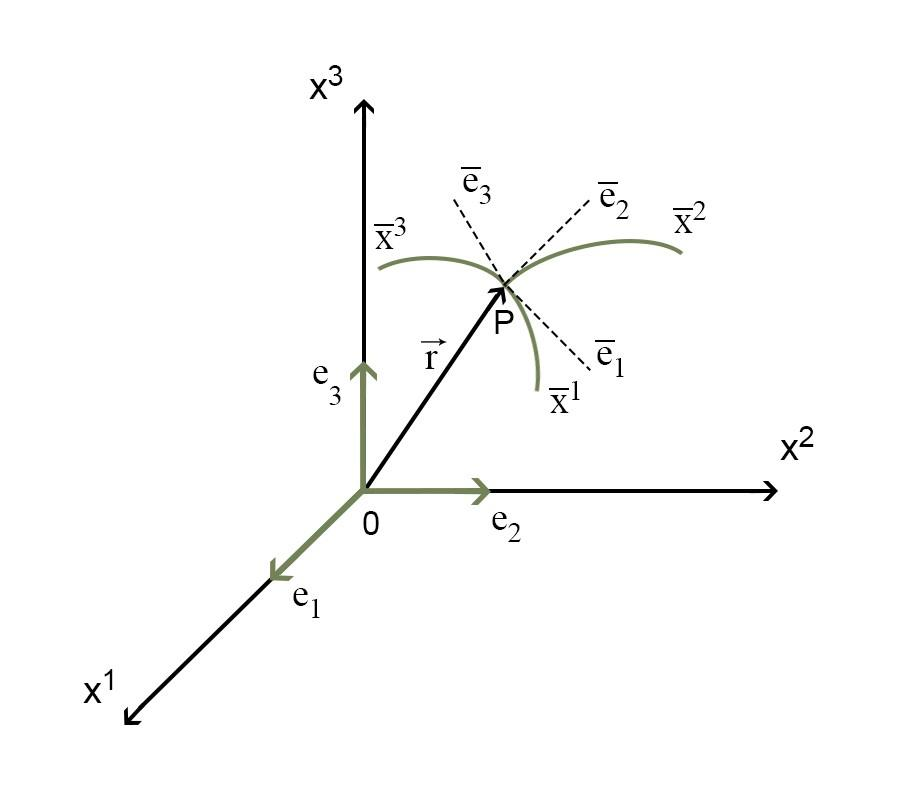
\includegraphics[scale=0.35]{Pictures/Tens_fig12.jpg}
\caption{Bases en coordenadas curvilíneas}
\label{Tens_fig12}
\end{center}
\end{figure}
 
  Las componentes del tensor métrico (representado por los elementos $ij$ de la matriz) son los productos escalares de los vectores  de la base $B^{\prime}$, es decir, $\overline {\bold{e}}_i \cdot \overline {\bold{e}}_j$ .
  
  \bigskip 
  
 Así, para el vector $\bold{v}=(1,1,1)_{B}$, se tiene
 
  \bigskip 
  
  \begin{equation}
\left(\begin{array}{ccc} 1 & 1 & 1 
\end{array}
 \right)_{B} \left(\begin{array}{ccc} 2  & 6  & 3   \\ 6 & 21  & 8 \\ 3   & 8 & 9
\end{array}
 \right)  \left(\begin{array}{c} 1 \\1  \\1
\end{array}
 \right)_{B}=  \left(\begin{array}{ccc} 11 & 35 & 20
\end{array}
 \right)\left(\begin{array}{c} 1 \\1  \\1
\end{array}
 \right)=66   \label{tensormej}
\end{equation}
 
 
 \bigskip
 
 Con esta definición nueva, (que da la longitud del vector elevada al cuadrado), el tensor métrico da la matriz identidad si la base es la canónica y se tiene el resultado presentado al inicio: 

  \begin{equation}
\left(\begin{array}{ccc} 7 & 4 & -1 
\end{array}
 \right) \left(\begin{array}{ccc} 1  & 0  & 0   \\ 0 & 1  & 0 \\ 0   & 0 & 1
\end{array}
 \right)  \left(\begin{array}{c} 7 \\4 \\-1
\end{array}
 \right)=  \left(\begin{array}{ccc} 7 & 4 & -1
\end{array}
 \right)\left(\begin{array}{c} 7 \\4  \\-1
\end{array}
 \right)=66   \label{tensormej2}
\end{equation}


\bigskip

De lo anterior surge que es posible  introducir  el concepto de distancia en un espacio $V$ de dimensión $N$ cualquiera, y que la distancia $ds$ entre dos puntos próximos de coordenadas $x^i$ y $x^i +dx^i$, está dada por la expresión:


\begin{equation}
\label{tmg}
ds^{2}=g_{ij}dx^{i}dx^{j}= g_{11}(dx^{1})^{2}+g_{12}dx^{1} dx^{2}+    \cdots + g_{1N}dx^{1}dx^{N} + \cdots +g_{NN}(dx^{N})^{2}
\end{equation}

\noindent 
donde  $g_{ij}$ son funciones de $x^i$, con la restricción que $g=\left | g_{ij} \right |\neq 0$. 

Cuando se cumple esta definición de longitud se dice que el espacio es un \textit{espacio de Riemann}. 


\begin{remark}
\begin{itemize}

\item
Se postula que la distancia entre dos puntos próximos es independiente del sistema de coordenadas, es decir que $ds$ es un \textit{invariante}. 

\item

A la forma cuadrática $  g_{ij}dx^{i}dx^{j}$ se la llama \textit{métrica}.   $ g_{ij}$  es un tensor simétrico covariante de segundo orden llamado \textit{tensor fundamental}.  Sus componentes contravariantes están dadas por los elementos de la matriz inversa.



\begin{equation}
g^{ij}g_{jk} =\delta^{i}_{k}
\end{equation}

\bigskip 




%Es decir que en un sistema de coordenadas curvilíneas $x^{i}$, la expresión  de la distancia  entre dos %puntos próximos de coordenadas $x^{i}$  y $x^{i} + \delta x^{i}$)   adopta la forma  diferencial %cuadrática

%\bigskip



\bigskip

Los coeficientes $g_{ij}$ son funciones de las coordenadas, y se obtienen a partir de  los vectores de la base, $\overline {\bold{e}}_{i}$, ya que 

\bigskip

\begin{eqnarray}\label{ec_9}
g_{ij}= \overline {\bold{e}}_{i}\cdot \overline {\bold{e}}_{j}
\end{eqnarray}
\bigskip

\item
$g_{ij}= g_{ji}$.  $ g_{ij} dx^{i} dx^{j}  $ es una forma cuadrática. Se llama  \textit{métrica}, y es el cuadrado del elemento de línea $ds$.

\item

%Se postula que la distancia entre dos puntos próximos es %independiente del sistema de coordenadas, es decir, $ds$ es un %invariante.
La longitud de los vectores de la base  viene dada por:

\begin{eqnarray}\label{ec_10}
\left| \overline {\bold{e}}_i\right| =\sqrt{g_{ii}}
\end{eqnarray}
donde $i$ no se suma en la última expresión. Además, si el sistema es ortogonal, $g_{ij}=0$ para $i\neq j$.

\item
En un espacio euclídeo de tres dimensiones, referido a un sistema de ejes cartesianos rectangulares se tiene que la expresión de la Ec.(\ref{tmg}) para tensores cartesianos para $N=3$, es

\begin{eqnarray}\label{ec_8}
ds^{2}= (dx^{1})^2+  (dx^{2})^2+(dx^{3})^2
\end{eqnarray}


\bigskip

Teniendo en cuenta que,
\begin{eqnarray*}
    \delta_{ij}=\delta_{i}^{j}=  
\left \{ \begin{array}{ll}
    1 &  \mbox{cuando $i=j$},  \\
    0  & \mbox{cuando $i \ne j$}
\end{array}
\end{eqnarray*}

\bigskip
\noindent
y desarrollando las sumas, 
\begin{eqnarray*}
\delta_{ij}x^ix^j&=&\delta_{1j}x^1x^j+ \delta_{2j}x^2x^j + \delta_{3j}x^3x^j\\
&=&\delta_{11}x^1x^1+\delta_{12}x^1x^2+ \delta_{13}x^1x^3+  \delta_{21}x^2x^1 + \delta_{22}x^2x^2 + 

+\delta_{23}x^2x^3 + \cdots +  \delta_{33}x^3x^3
\end{eqnarray*}

\bigskip

$\delta_{ij}x^ix^j= (x^{1})^{2}+(x^{2})^{2}+(x^{3})^{2}= ds^{2}$

\bigskip

\begin{remark}
 Las expresiones  $\delta_{ij}x^ix^j=\delta_{m l}x^m x^l=\delta_{\beta \alpha}x^\beta x^\alpha$ son equivalentes por ser los índices mudos.
\end{remark}

\bigskip

%Notar que el índice repetido puede cambiarse a voluntad sin que se altere el resultado, mientras que el %índice que se presenta sólo una vez, no puede cambiarse. Así el índice repetido (índice mudo), %desaparece una vez efectuada la suma, y el que no se repite, queda presente en la expresión (índice %libre).
%Por ejemplo,

%\bigskip

%$\delta_{j}^{i}x^j= \delta_{1}^{i}x^1+ \delta_{2}^{i}x^2+ \delta_{3}^{i}x^3=x^{i}$

%\bigskip







%\item


%\begin{equation}
%ds^{2}=(dx^{1})^{2}+(dx^{2})^{2}+(dx^{3})^{2}
%\end{equation}
El tensor métrico en este caso es 

$$g_{ij}=\left(\begin{array}{ccc} 1 & 0 & 0 \\  0 & 1 & 0 \\ 0  & 0 & 1
\end{array}
 \right)$$



\bigskip



Las componentes del tensor fundamental son cero, excepto $g_{11}=g_{22}=g_{33}=1$.





    \item 
    La métrica en un espacio euclídeo es positiva. Será cero solo cuando $ dx^{1}= dx^{2} =dx^{3}=0 $.
    
    \item 
    En la teoría especial de la relatividad  la métrica no siempre es positiva. Su expresión está dada por

\begin{eqnarray}\label{ec_8}
ds^{2}=-  (dx^{1})^2-  (dx^{2})^2- (dx^{3})^2 + c^{2}(dx^{4})^2
\end{eqnarray}
\bigskip
\item
   Otro ejemplo de métrica en un espacio euclídeo es la referida  a coordenadas polares esféricas   $ x^{1}=r $, $ x^{2}=\theta $  y $ x^{3}=\psi $. La métrica está   dada por 
   
 \begin{eqnarray}\label{ec_8}
ds^{2}=  dr^{2}+ r^{2} d\theta^{2}+ r^2 sen^{2}\theta d\psi^2
\end{eqnarray}
 
    
    
    \end{itemize}
    %\hfill$\blacktriangle$
\end{remark}

%\newpage
\noindent Ejemplos de diferentes métricas:\\

De acuerdo con la teória de la relatividad general en presencia de materia, la geometría del espacio-tiempo no es plana. La métrica de Schwarzchild describe como se curva el espacio-tiempo a causa de un cuerpo esférico, aislado y estático que no gira sobre si mismo ($r$: distancia, $G$: constante gravitatoria, $M$: Masa, $c$: velocidad de la luz y $\theta$= ángulo):\\

Métrica de Schwarzchild: 

\bigskip

$g_{ij}= \left(\begin{array}{cccc}  -c^2(1- \frac{2GM}{c^2 r}) & 0 & 0& 0 \\ 0 &  (1- \frac{2GM}{c^2 r})^{-1}& 0 & 0 \\   0 & 0 & r^2 &0 \\ 0 & 0 & 0 & r^2sen^2(\theta)

\end{array}
 \right)  \qquad $

 \bigskip

 Por otro lado la métrica de Friedman-Lamaitre-Roberson-Waller nos describe la expansión de universo en términos del parámetro $k$. Si $k>0$ el universo es cerrado y volverá a plegarse sobre sí mismo generando un nuevo bigbang (teoría del bigcrush), mientras que si $k\leq 0$ el universo se expande sin límites. ($a(t)$ representa la aceleración del universo):\\

 Métrica de FLRW: 
 
 \bigskip
 
 $g_{ij}= \left(\begin{array}{cccc}  -c^2 & 0 & 0& 0 \\ 0 &  a(t)(\frac{1}{1-kr^2 })& 0 & 0 \\   0 & 0 & a(t)(\frac{1}{1-kr^2 }) &0 \\ 0 & 0 & 0 & a(t)r^2sen^2(\theta)(\frac{1}{1-kr^2 })

\end{array}
\right)  \qquad $






\subsection{Bases en coordenadas curvilíneas.}
\bigskip

%\textbf{Bases covariantes}
%\begin{eqnarray}\label{ec_4}
%e_{\theta}= \frac {\partial  \vec r}{\partial \theta}=  lim_{\Delta \theta \rightarrow 0} \frac {\vec r (P, \theta+\Delta \theta, \varphi)-\vec r (P, \theta, %\varphi) }{\Delta \theta} %
%\end{eqnarray}



\bigskip

De acuerdo a la Figura \ref{Tens_fig12},

\begin{eqnarray}\label{ec_5}
\bold{r} = x^{1}  \bold{e}_{1} +  x^{2}  \bold{e}_{2}+  x^{3}  \bold{e}_{3}
\end{eqnarray}



\bigskip
\noindent
donde \[ \bold{e}_{j}= \frac {\partial  \bold{r}}{\partial x^{j}}\]

\bigskip

Para cada punto $P$ del espacio se tienen tres líneas coordenadas $  \overline x^{i}$; es posible definir  tres vectores base para $P$ como:

\begin{eqnarray}\label{ec_6}
\overline {\bold{e}}_{i}= \frac {\partial  \bold{r}}{\partial \overline x^{i}}
\end{eqnarray}

\bigskip
\noindent
que se llaman vectores tangentes a las lineas coordenadas (\cite{itskov}) $  \overline x^{i}$. 
%En ec.\ref{ec_4} y Figura $3$ observamos  el procedimiento en virtud del cual se obtiene $e_{\theta}$, tangente a la línea coordenada $\theta$ %(semicircunferencia), en coordenadas esféricas.

\vskip.5cm

La base $\overline {\bold{e}}_{i}$, representada en la Figura \ref{Tens_fig12} es, en general, variable punto a punto y sus versores no necesariamente tienen longitud unitaria. Se trata de una base \textit{local }; cada punto $P$ del espacio tiene su propia base.






En un sistema de coordenadas curvilíneas  se tiene, en cada punto $P$, una base local dada por   los vectores  $\overline {\bold{e}}_{i}$ de  la Ec.(\ref{ec_6}) como se muestra en la Figura \ref{Tens_fig12}. De ahora en adelante a los vectores de esta base   los denotaremos $ \bold{g}_i$.


\bigskip

\begin{example} Coordenadas cilíndricas


\begin{eqnarray}\label{ec_19}
\vec r = x^{1}  \bold{e}_{1} +  x^{2}  \bold{e}_{2}+  x^{3}  \bold{e}_{3}
\end{eqnarray}
\vskip.25cm
donde $x^{1}=r cos(\varphi)$, $x^{2}=r sen(\varphi)$ y $x^{3}=z$

\bigskip
Es una transformación entre las coordenadas $x^{i} $ y,  $\overline x^{i}$

\bigskip

 $\overline x^{1}=r$, $\overline x^{2}=\varphi$ y $\overline x^{3}=z$


\bigskip





%De acuerdo a la ec.(\ref{ec_15}), despejando  


%\begin{eqnarray}\label{ec_25}
%  \vec{ g}_{i}= \frac {\partial   x^{j}}{\partial \overline x^{i}} \vec{e}_{j}  
%\end{eqnarray}



Los vectores tangentes (o base covariante, Ec.(\ref{ec_6})), son 

\bigskip

\begin{eqnarray}\label{ec_20}
\bold{g}_{1}= \frac {\partial  \bold{r}}{\partial \overline x^{1}}=cos(\varphi)  \bold{e}_{1} + sen(\varphi)  \bold{e}_{2}+  0. \bold{e}_{3}
\end{eqnarray}
\vskip.25cm
\begin{eqnarray}\label{ec_21}
 \bold{g}_{2}= \frac {\partial  \bold{r}}{\partial \overline x^{2}}=-r sen(\varphi)  \bold{e}_{1} +r  cos(\varphi)   \bold{e}_{2}+  0. \bold{e}_{3}
\end{eqnarray}

\bigskip

\begin{eqnarray}\label{ec_22}
 \bold{g}_{3}= \frac {\partial  \bold{r}}{\partial \overline x^{3}}=0  \bold{e}_{1} + 0   \bold{e}_{2}+  1  \bold{e}_{3}
\end{eqnarray}

\bigskip
\end{example}


%\textbf{Bases recíprocas (o duales)}

Existe además, para cada punto $P$, otro conjunto de tres direcciones  que puede ser adoptado para definir otra base local de vectores que  denotaremos  por $\bold{g}^{i}$.


\bigskip

Estos vectores $\bold{g}^{i}$  constituyen la denominada \textit{base recíproca o dual  } de la $\bold{g}_{i}$, en virtud de las relaciones:


\begin{eqnarray}\label{ec_11}
\bold{g}^{i}\cdot \bold{g}_{j}=\delta _{j} ^{i} 
\end{eqnarray}


%\noindent
Pueden obtenerse de la forma siguiente
\begin{eqnarray}\label{ec_12}
\bold{g}^{1}= \frac {\bold{g}_{2}\times \bold{g}_{3} }{\left[  \bold{g}_{1}\bold{g}_{2} \bold{g}_{3} \right]} \qquad
\bold{g}^{2}= \frac {\bold{g}_{3}\times \bold{g}_{1} }{\left[  \bold{g}_{1}\bold{g}_{2} \bold{g}_{3} \right]} \qquad
\bold{g}^{3}= \frac {\bold{g}_{1}\times \bold{g}_{2} }{\left[  \bold{g}_{1}\bold{g}_{2} \bold{g}_{3} \right]} 
\end{eqnarray}

\bigskip

\noindent
donde $\left[  \bold{g}_{1}\bold{g}_{2} \bold{g}_{3} \right]=\bold{g}_{1}\times \bold{g}_{2} \cdot \bold{g}_{3}=E  $ 

\bigskip

En la Figura \ref{Tens_fig2} se muestra un ejemplo en cartesianas.

Y también, 

\bigskip

\begin{eqnarray}\label{ec_13}
\bold{g}_{1}= \frac {\bold{g}^{2}\times \bold{g}^{3} }{\left[  \bold{g}^{1}\bold{g}^{2} \bold{g}^{3} \right]} \qquad
\bold{g}_{2}= \frac {\bold{g}^{3}\times \bold{g}^{1} }{\left[  \bold{g}^{1}\bold{g}^{2} \bold{g}^{3} \right]}  \qquad
\bold{g}_{3}= \frac {\bold{g}^{1}\times \bold{g}^{2} }{\left[  \bold{g}^{1}\bold{g}^{2} \bold{g}^{3} \right]} 
\end{eqnarray}

\bigskip

\noindent
y $\left[  \bold{g}^{1}\bold{g}^{2} \bold{g}^{3} \right]=E_R$



 



%\bigskip

%\begin{eqnarray}\label{ec_122}
%\bold{g}^{3}= \frac {\bold{g}_{1}\times \bold{g}_{2} }{\left[  \bold{g}_{1}\bold{g}_{2} \bold{g}_{3} \right]} 
%\end{eqnarray}

\bigskip


De la misma forma que en Ec.(\ref{ec_9}), se tiene 

\bigskip

\begin{eqnarray}\label{ec_14}
g^{ij}= \bold{g}^{i}\cdot \bold{g}^{j}
\end{eqnarray}


\bigskip
\noindent
y naturalmente,  $g^{ij}= g^{ji}$

\bigskip

\begin{figure}
%\centering
\begin{center}
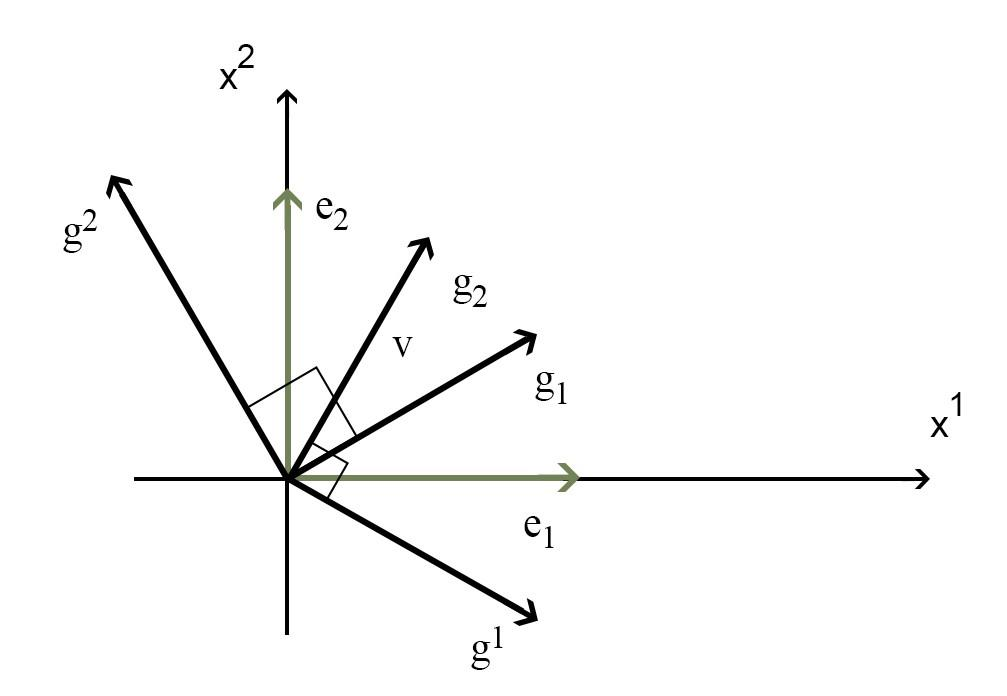
\includegraphics[scale=0.4]{Pictures/Tens_fig2.jpg}
\caption{Ejemplo de una base $\bold{g}_{i}$ y su base recíproca $\bold{g}^{j}$}
\label{Tens_fig2}
\end{center}
\end{figure}

Decimos que estas dos bases, que son mutuamente recíprocas, y se pueden demostrar las siguientes propiedades

\bigskip

\begin{itemize}
\item
$\left[  \bold{g}_{1}\bold{g}_{2} \bold{g}_{3} \right]\left[  \bold{g}^{1}\bold{g}^{2} \bold{g}^{3} \right]=1 \qquad  E_R= E^{-1}  $

\bigskip
\item

det($g_{ij})=g=E^{2} \qquad  E=\sqrt{g}  $

\bigskip

\item

$g^{ik}g_{kj}=\delta^{i}_{j}$

\bigskip
\item
$\bold{e}^{j}\times \bold{e}_{j}=0$
\end{itemize}

\bigskip


En un sistema cartesiano ortogonal, la base recíproca  coincide con aquella que la genera, es decir, $\bold{g}^{i}= \bold{g}_{i} $.

\bigskip

\begin{example} \textbf{Coordenadas cilíndricas.}\index{Coordenadas cilíndricas}


La base recíproca, usando ec.(\ref{ec_12})



\begin{eqnarray}\label{ec_32}
 \bold{g}^{1}= \frac {\bold{g}_{2}\times \bold{g}_{3} }{\left[  \bold{g}_{1}\bold{g}_{2} \bold{g}_{3} \right]} 
\end{eqnarray}


\begin{eqnarray}\label{ec_29}
 \bold{g}^{1} = ( r cos(\varphi)  \bold{e}_{1} + r sen (\varphi)  \bold{}{e}_{2}+  0  \bold{e}_{3})/ r 
\end{eqnarray}

\begin{eqnarray}\label{ec_31}
\bold{g}^{2} = ( - sen(\varphi)  \bold{e}_{1} + cos (\varphi)  \bold{e}_{2}+  0  \bold{e}_{3})/ r 
\end{eqnarray}

\begin{eqnarray}\label{ec_33}
\bold{g}^{3} = ( r cos^{2}(\varphi)  \bold{e}_{1} +  r  sen^{2}(\varphi)  \bold{e}_{2}+  0  \bold{e}_{3})/ r 
\end{eqnarray}

\bigskip









En la Figura \ref{Tens_fig3} se muestran las coordenadas cilíndricas en el espacio $\mathbb{R}^{3}$ y los vectores $\overline {g}_{i}$.













%\begin{eqnarray}\label{ec_15}
%e_{j}= \frac {\partial  \overline x^{i}}{\partial  x^{j}}\overline e_{i}  
%\end{eqnarray}

\bigskip


Como por la Ec.(\ref{ec_9}),  $g_{ij}= g_{i}\cdot g_{j}$

\bigskip

 $g_{11}= \bold{g}_{1}\cdot \bold{g}_{1}=cos^{2}(\varphi)  + sen^{2}(\varphi)=1$

\bigskip

 $g_{12}= \bold{g}_{1}\cdot \bold{g}_{2}=-r cos(\varphi) sen(\varphi) +r cos(\varphi) sen(\varphi) =0 $
\bigskip

 $g_{13}= \bold{g}_{1}\cdot \bold{g}_{3}=0 $
\bigskip

 $g_{22}= \bold{g}_{2}\cdot \bold{g}_{2}=r^{2} sen ^{2}(\varphi) +r^{2} cos^{2}(\varphi) = r^{2}$
\vskip.25cm

 $g_{23}= \bold{g}_{2}\cdot \bold{g}_{3}=0 $
\vskip.25cm

 $g_{33}= \bold{g}_{3}\cdot \bold{g}_{3}=1 $
\vskip.25cm


$$g_{ij}= \left(\begin{array}{ccc}  1 & 0 & 0 \\ 0 &  r^{2} & 0 \\   0 & 0 & 1
\end{array}
 \right)$$
\vskip.25cm
y su inversa
\vskip.25cm
$$g^{ij}= \left(\begin{array}{ccc}  1 & 0 & 0 \\ 0 &  r^{-2}  & 0 \\   0 & 0 & 1
\end{array}
 \right)$$

\end{example}



\textbf{Relaciones entre versores de  base}

\bigskip

Dados dos sistemas de coordenadas curvilíneas  $ x^{i}$, $\overline x^{i}$, y considerando para cada uno de ellos las bases anteriormente introducidas, existen entre sus versores las relaciones:

\bigskip

\begin{eqnarray}
\label{ec_15}
\bold{g}_{j}= \frac {\partial  \overline{x}^{i}}{\partial  x^{j}} { \overline{\bold{g}}_{i} \qquad   \qquad  \overline{\bold{g}}_{i}= \frac {\partial  x^{j}}{\partial \overline{x}^{i}} \bold{g}_{j}  
\end{eqnarray}

\bigskip

\begin{eqnarray}\label{ec_16}
\bold{g}_{i}= g_{ij}\bold{g}^{j}  \qquad   \qquad  \bold{g}^{i}= g^{ij}\bold{g}_{j}
\end{eqnarray}
\vskip.25cm

Si
\begin{eqnarray}\label{ec_18}
 \bold{g}^{k} = \frac {\partial  x^{k}}{\partial \overline x^{j}} \overline {\bold{g}}^{j}, \qquad   \qquad  
 \overline {\bold{g}}^{j} = \frac {\partial \overline x^{k}}{\partial  x^{j}}  \bold{g}^{j}
\end{eqnarray}

\begin{eqnarray}\label{ec_17}
 \bold{g}_{m} = \frac {\partial  x^{i}}{\partial \overline x^{j}}g_{mi} \overline {\bold{g}}^{j}, 
\end{eqnarray}
\noindent 
se tiene que esta expresión se demuestra de la forma siguiente:


\noindent 
usando Ec.(\ref{ec_15})

$$\bold{g}_{m}= \frac {\partial  \overline x^{i}}{\partial  x^{m}}\overline {\bold{g}}_{i}  $$



$$\bold{g}_{m}= \frac {\partial  \overline x^{i}}{\partial  x^{m}} \frac {\partial  x^{j}}{\partial \overline x^{i}} \bold{g}_{j} $$ 

Reemplazando la Ec.(\ref{ec_16})

$$\bold{g}_{m}= \frac {\partial  \overline x^{i}}{\partial  x^{m}} \frac {\partial  x^{j}}{\partial \overline x^{i}} g_{jk} \bold{g}^{k} $$ 

Teniendo en cuenta la  Ec.(\ref{ec_18})
\vskip.25cm
$$\bold{g}_{m}=  \frac {\partial  x^{j}}{\partial \overline x^{i}} \frac {\partial  \overline x^{i}}{\partial  x^{m}} g_{jk}  \frac {\partial  x^{k}}{\partial \overline x^{j}} \overline {\bold{g}}^{j} $$ 

\bigskip

\noindent
y como  $\frac {\partial  x^{j}}{\partial \overline x^{i}} \frac {\partial  \overline x^{i}}{\partial  x^{m}}= \delta^j_m$, se tiene que 
$$\bold{g}_{m}=  \delta^j_m g_{jk}  \frac {\partial  x^{k}}{\partial \overline x^{j}} \overline {\bold{g}}^{j} $$ 


$$\bold{g}_{m}=  \frac {\partial  x^{k}}{\partial \overline x^{j}}  g_{mk}   \overline {\bold{g}}^{j},$$ 

\bigskip
\noindent
que coincide con Ec.(\ref{ec_17}) ya que  $k$ es un índice mudo.

\begin{figure}
%\centering
\begin{center}
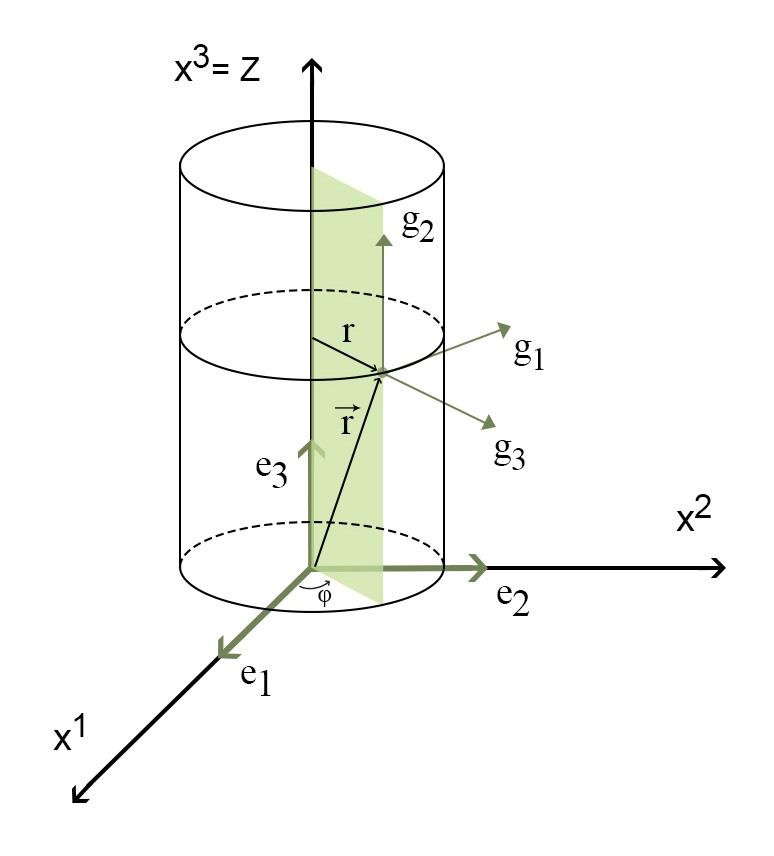
\includegraphics[scale=0.4]{Pictures/Tens_fig3.jpg}
\caption{Coordenadas cilíndricas}
\label{Tens_fig3}
\end{center}
\end{figure}

\bigskip





\textbf{Componentes contravariantes y covariantes de un tensor}


De lo anterior surge que dado un tensor  $\bold A$ se dispone de dos bases aptas para su expresión: la $\bold{g}_{i}$ y su recíproca $\bold{g}^{j}$. Las componentes de $\bold A$ en $\bold{g}_{i}$ las denominamos \textit{contravariantes} y las indicaremos $A^{i}$, mientras que las componentes en $\bold{g}^{j}$ las llamaremos \textit{covariantes}, designándolas $A_{j}$. Entonces:

\begin{eqnarray}\label{ec_19ap}
\bold A=   A^{i}\bold{g}_{i}=  A_{j}\bold{g}^{j}
\end{eqnarray}

\bigskip





Como se mencionó antes, si el sistema es cartesiano ortogonal, ambas componentes son indistinguibles: $A^{i}=A_{i} $. Cuando $\bold A$ esté dado mediante $A^{i}$, diremos \textit{vector contravariante}; o vector  covariante $A_{k} $ si se nos presenta mediante esas componentes. Entre ellas se cumple:

\bigskip

\begin{eqnarray}\label{ec_20ap}
A_j=   g_{ij}  A^{i} \qquad  A^{j}=g^{ij}A_i
\end{eqnarray}

\bigskip

así, $g_{ij}$ y    $g^{ij}$ bajan y suben índices, respectivamente.
\vskip.25cm




Para demostrarlo, por ejemplo, la primera igualdad,  partimos de la expresión

$$ \bold A= A_k ~\bold{g}^k = A^l ~ \bold{g}_l $$

Multiplicando  escalarmente por $\bold{g}_j$  a ambos lados,

$$  A_k ~ \bold{g}^k \cdot \bold{g}_j = A^l ~ \bold{g}_l \cdot \bold{g}_j$$


y teniendo en cuenta la relación entre los vectores de la base y de su base recíproca, Ec.(\ref{ec_11}),


$$  A_k ~ \delta^{k}_j = A^i ~ \bold{g}_i ~ \bold{g}_j$$


 y se obtiene 
 
 $$A_j=   g_{ij}  A^{i}$$

\bigskip

Entre las componentes contravariantes (o duales) de $\bold A$ en dos sistemas $x^i$, $\overline x^i$ se verifica:



\bigskip
\begin{eqnarray}\label{ec_21ap}
A^{i} = \frac{\partial  x^i}{\partial \overline x^j} \overline A^{j}  \qquad \overline  A^{j}=\frac{\partial \overline x^j}{\partial  x^i} \overline A^{i} 
\end{eqnarray}

\bigskip

\noindent
y entre las covariantes

\bigskip

\begin{eqnarray}\label{ec_22ap}
A_{i} = \frac{\partial \overline x^j}{\partial  x^i} \overline A_{j}  \qquad \overline  A_{k}=\frac{\partial  x^j}{\partial \overline x^k} \overline A_{j} 
\end{eqnarray}

\bigskip

y además, 
\bigskip
\begin{eqnarray}\label{ec_23ap}
A^{j} = \bold A \cdot \bold{g}^j  \qquad  A_{i} = \bold A \cdot \bold{g}_i 
\end{eqnarray}
\vskip.25cm




De lo anterior sale que una vez  definido el tensor métrico, las  componentes covariantes y contravariantes de un tensor  están relacionadas por el tensor métrico, así por ejemplo,


$$v^{i}=g^{ij}v_{j}$$
$$v_{l}=g_{lm}v^{m}$$
$$T^{ij}=g^{il}T_{l}^{j}=g^{il}g^{jm}T_{lm}$$




Es importante notar que bases definidas ($\bold{g}_{i}$ y su recíproca $\bold{g}^{i}$) cumplen la relación de la Ec.( \ref{ec_11}) y que esta relación se mantiene al realizar una transformación de coordenadas.Para demostrarlo, se utilizan   los vectores contravariantes y covariantes, $\overline{\bold{g}}^{i} $ y $\overline{\bold{g}}_{j} $, y sus relaciones con los vectores $\bold{g}^{i} $ y $\bold{g}_{j} $, respectivamente  (Ecs.(\ref{contravariante}) y (\ref{covariante})). Se verá  que $\overline{\bold{g}}^{i} \cdot \overline{\bold{g}}_{j} = \delta^i_{~j} $.


\begin{eqnarray}\label{demdelta}
\overline{\bold{g}}^{i} \cdot \overline{\bold{g}}_{j}&=& \frac{\partial \overline x^i}{\partial  x^l}  \bold{g}^{l} \cdot \frac{\partial  x^k}{\partial \overline x^j} \bold{g}_{k} \\
&= &\frac{\partial \overline x^i}{\partial  x^l}  \frac{\partial  x^k}{\partial \overline x^j} \bold{g}^{l} \cdot \bold{g}_{k} \\
&=& \frac{\partial \overline x^i}{\partial  x^l}  \frac{\partial  x^k}{\partial \overline x^j} \delta^{l}_{~k}\\
&=& \frac{\partial \overline x^i}{\partial  x^l}  \frac{\partial  x^l}{\partial \overline x^j}\\
&=&  \delta^{i}_{~j}\\
\end{eqnarray}

\textbf{Componentes físicas de un vector}
En ciertos contextos son importantes las componentes físicas de un vector. Si $ \bold A= A^l  g_l $, están dadas por 

$$  \left |A^l \right |   \left |\bold{g}_l \right |  = \left |A^l \right | \sqrt{g_{jj}}$$





\section{Diagonalización de tensores de segundo orden. Invariantes.}

Dado un tensor de segundo orden simétrico y real siempre existe un sistema de coordenadas en el cual las únicas componentes no nulas del tensor son las que tienen los dos índices iguales, $t_{ij}=0$  si $i \neq j$. 
Si $T$ es la matriz de los $t_{ij}$, $T$ es una matriz diagonal:

$$T= \left(\begin{array}{ccc}  t_{11}& 0 & 0 \\ 0 &  t_{22} & 0 \\   0 & 0 & t_{33}
\end{array}
 \right)$$
\noindent
(para N=3).
El sistema de coordenadas en el que el tensor es diagonal se llama de \textit{ejes principales}.

Para demostrar que todo tensor simétrico y real es diagonalizable, se hace el producto escalar del tensor de componentes $t_{ij}$ por un vector $\textbf{v}_i$, con lo que se obtiene otro vector   $\textbf{w}_i$:
$$\textbf{w}_i= t_{ij}\textbf{v}_j.$$
Se trata de hallar los vectores $\textbf{v}_i$ tales que el vector resultante sea un múltiplo, o sea 
$$\textbf{w}_i= \lambda  \textbf{v}_i   \qquad   i=1,2, \cdots N.$$
donde   $ \lambda$ es un escalar. En ese caso a $\textbf{v}_i$ se lo llama \textit{autovector} y a  $ \lambda$  \textit{autovalor}.

Para que esto suceda los vectores $\textbf{v}_i$ deben satisfacer 

$$t_{ij}\textbf{v}_j= \lambda  \textbf{v}_i  $$


o
$$(t_{ij}- \lambda \delta_{ij})\textbf{v}_j= \vec{0}  $$

%$$T( \vec v)= \lambda \vec v$$




Para el caso que $N=3$, se tiene  un sistema de  ecuaciones  algebraicas:


\begin{equation} \label{diagT}
\left\{ \begin{array} {ccl} 
                    (t_{11}-\lambda)\textbf{v}_1+t_{12}\textbf{v}_2 +t_{13}\textbf{v}_3  =& 0  \\
                    t_{21}\textbf{v}_1+(t_{22}-\lambda)\textbf{v}_2+t_{23}\textbf{v}_3 =& 0 \\
                    t_{31}\textbf{v}_1+t_{32}\textbf{v}_2+(t_{33}-\lambda)\textbf{v}_3  =& 0
                   \end{array}
           \right.
\end{equation}



\bigskip

Como es un sistema homogéneo, para que tenga solución no trivial el determinante del sistema debe ser nulo.
A la ecuación
\begin{equation}
\label{eccaractT}
 det(T- \lambda I)=0   
\end{equation}


\noindent
se la llama ecuación característica  del tensor $\mathbf{T}$. 





El determinante de la Ec.(\ref{eccaractT}) es un polinomio de grado $3$ con respecto  a las potencias de $\lambda$:


%$$ P_T(\lambda) = (-1)^n \lambda^n + (-1)^{n-1} \lambda^{n-1} \mathbf{I_T}^{(1)} +  \cdots +  (-1)^{n-k} \lambda^{n-k} \mathbf{I_T}^{(k)} %+ \cdots + \mathbf{I_T}^{(n)}$$


 $$ P_T(\lambda) =  \lambda^3 +  \lambda^{2} \mathbf{I_T} + \lambda \mathbf{II_T} - \mathbf{III_T}=0$$
\noindent 
llamado polinomio característico del tensor $\mathbf{T}$. $\mathbf{I_T}$, $\mathbf{II_T}$, $\mathbf{III_T}$ son los \textit{invariantes principales} del tensor $\mathbf{T}$, definidos en función de sus componentes $t_{ij}$ por  (ver \cite{chaves}):

$$\mathbf{I_T}=tr(\mathbf{T})=t_{ii}$$

$$\mathbf{II_T}=\frac{1}{2} [ tr(\mathbf{T})^2-tr(\mathbf{T}^2)]$$


$$\mathbf{III_T}=Det(\mathbf{T})$$


Si $\mathbf{T}$ es un tensor simétrico, los invariantes principales se resumen de la forma:

\bigskip

$\mathbf{I_T}=t_{11}+t_{22}+t_{33}$

$\mathbf{II_T}=t_{11}t_{22} +t_{11}t_{33}+ t_{22}t_{33}- t_{12}^2 -t_{13}^2-t_{23}^2  $


$\mathbf{III_T}=t_{11}t_{22}t_{33}+ t_{12}t_{13}t_{23} +t_{13}t_{12}t_{23}- t_{12}^2 t_{33} -t_{23}^2 t_{11}-t_{13}^2 t_{22} $



\begin{remark}
\begin{itemize}
\item
Encontrar los autovalores o valores principales es equivalente a encontrar unas direcciones principales (autovectores) tales que $t_{ij}=0$ para $i \neq j$.


\item
 Una vez obtenidos los autovalores, los autovectores se obtiene  resolviendo las ecuaciones 

 $(t_{ij}- \lambda_1 \delta_{ij}) \textbf{n}_j^{(1)}=\Vec{0}$, $~(t_{ij}- \lambda_2 \delta_{ij}) \textbf{n}_j^{(2)}=\Vec{0}$ y $~(t_{ij}- \lambda_3 \delta_{ij}) \textbf{n}_j^{(3)}=\Vec{0}$.
\item
Si $\mathbf{T}$ es un tensor simétrico el espacio de los autovectores está definido por una base ortonormal y los autovalores son todos reales.


\item

Cuando un tensor presenta los tres autovalores iguales,  $\lambda_1= \lambda_2= \lambda_3$ se denomina \textit{Tensor Esférico}.
\end{itemize}
\end{remark}
\section{Tensores de mayor orden}

Hemos visto tensores de órdenes $0$, $1$ y $2$. De la misma forma es posible definir tensores de orden mayor. 

Un conjunto de $N^{s+p}$ funciones  $A^{t_1 t_2 \cdots  t_s}_{q_1 q_2 \cdots  q_p}$ de las $N$ coordenadas $x^i$ se dice que son las componentes de un \textit{tensor mixto} de orden $(s+p)$ contravariante de orden $s$ y covariante de orden $p$ si se transforman según la ecuación


\bigskip

\[\overline{A}^{u_1 u_2 \cdots  u_s}_{r_1 r_2 \cdots  r_p}=   \frac{\partial \overline{x}^{u_1}}{\partial  x^{t_1} }  \cdots  \frac{\partial \overline{x}^{u_s}}{\partial  x^{t_s} }  \frac{\partial  x^{q_1}}{\partial \overline {x}^{r_1}} \cdots \frac{\partial  x^{q_p}}{\partial \overline {x}^{r_p}}  A^{t_1 t_2 \cdots  t_s}_{q_1 q_2 \cdots  q_p}\]

\bigskip
\noindent
con el cambio de coordenadas $x^i $ en $\overline{ x}^i $.

  Aunque esta expresión parece complicada  es simplemente una combinación de la Ec.(\ref{contravariante} )  con respecto a los índices contravariantes y de la Ec.(  \ref{covariante}) en cuanto a los índices covariantes.

\bigskip


Un ejemplo de orden $4$ es el \textit{tensor constitutivo} $\bold C$ que relaciona las componentes de dos tensores de orden $2$, el \textit{tensor de deformaciones}, $\bold{\epsilon}$ con el \textit{tensor de tensiones},  $\bold{\tau}$.


$$ \tau_{ij}= {C}_{ijkl} \epsilon_{kl}  $$

El tensor constitutivo $C_{ijkl}$ es de orden  $4$ y sus componentes, considerando dos bases ortogonales $e_i$ y $\overline e_j$ del sistema cartesiano,  se transforman de la forma siguiente

$$\overline{ C}_{ijkl}= p_{im}p_{jn}p_{kr}p_{ls}   {C}_{mnrs} \epsilon_{kl}   $$


\begin{remark}
En las  ecuaciones de elasticidad para  el estudio de tensiones y deformaciones en cáscaras y láminas es muy útil expresar  el tensor constitutivo en las componentes de una base local no ortogonal. Se utilizan las bases de vectores  covariantes y contravariantes.
%\hfill$\blacktriangle$
\end{remark}

\bigskip






\begin{parchment}[Juan Martín Maldacena]\index{Maldacena, Juan Martín}
{Nacido en Buenos Aires, 10 de septiembre de 1968. Entre sus muchos aportes al campo de la teoría de supercuerdas —o Teoría M—, se encuentra la denominada «conjetura de Maldacena», «dualidad de Maldacena» o correspondencia AdS/CFT, que propone la equivalencia entre ciertas teorías de gravedad cuántica y cualquier teoría conforme de campos bajo determinadas condiciones que satisfacen el principio holográfico. En 1997 se unió a la Universidad de Harvard como profesor asociado —entonces el profesor asociado vitalicio más joven de la historia de Harvard—. Ahí en 1999 ascendió a profesor titular. En 2012 fue honrado con el nuevo Premio Yuri Milner a la física fundamental. La distinción le dotó con tres millones de dólares. En ese momento sus investigaciones estaban orientadas a la relación entre espacio y tiempo cuánticos y a las teorías de partículas. En 2018 recibió la Medalla Lorentz siendo así el único científico de habla hispana y de Iberoamérica en haberla recibido. \cite{Malda}}
\end{parchment}

\bigskip


\newpage


\begin{figure}
%\centering
\begin{center}
%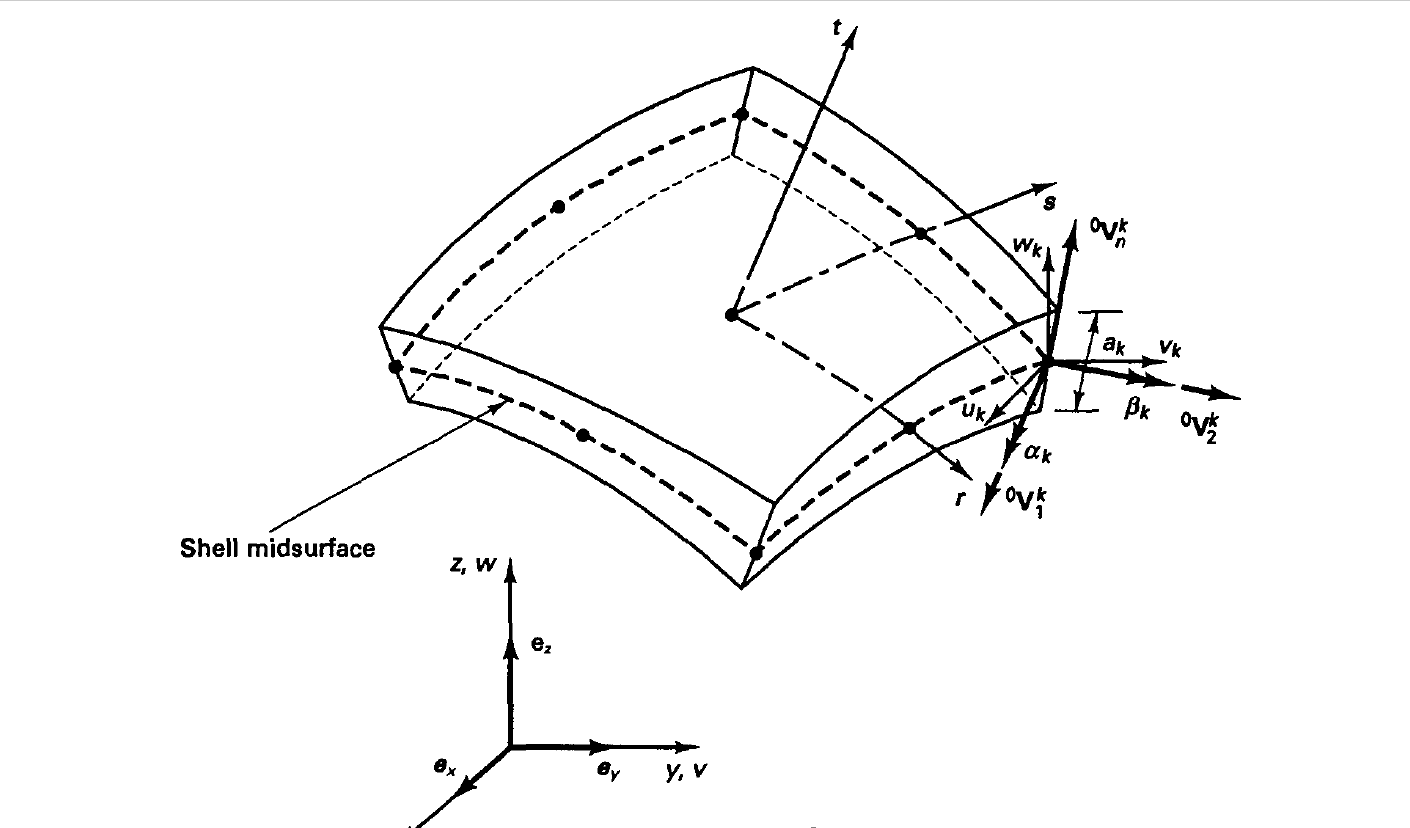
\includegraphics[scale=0.55]{Pictures/FIGURA150.png}
\end{center}
\end{figure}
%\begin{figure}
%\label{figproyxy}
    %\centering
    %
\includegraphics[width=0.60\textwidth]{Pictures/tensor.png}    
    %\label{TLfig13}
%\end{figure}
\section{Actividades propuestas}
%\section{Ejercitación}
\begin{answers}
Para el sistema de coordenadas esféricas \index{Coordenadas esféricas}

\bigskip
 
 $\vec{r}(\varphi,\phi,r)=r sen(\varphi)sen(\phi)\bold{e}_1+rcos(\phi)\bold{e}_2+rcos(\varphi)sen(\phi)\bold{e}_3$
 
  halle:
  
  \bigskip
  
 \noindent a) Los vectores base covariantes.
 
 \bigskip
 
  b)  Los vectores base contravariantes.
  
  \bigskip
  
  c) La métrica del sistema del coordenadas.

  \bigskip
  
  d) La matriz Jacobiana de la transformación  de coordenadas.
  
  \bigskip
  
  e) Calcule el $ds^{2}$  del sistema de coordenadas  $(\varphi,\phi,r)$. 
\end{answers}

\subsection{Ejercicios}

\bigskip

%\subsubsection{Notación Tensorial.}

 \vspace{0.5 cm}

 \begin{exercise}

\item

Responda:

a) ¿Qué información  dan los subíndices libres?

b) ¿Cómo se identifican los subíndices mudos?

c) ¿Por qué se llama frecuentemente a la delta de Kronecker operador de sustitución?

d) ¿Qué valor toma la terna 132 para el símbolo de permutación?

\end{exercise}


\begin{exercise}
\item 

Reescriba usando notación indicial las siguientes expresiones:
\begin{enumerate}
  
\item

$a_1x_1x_3+ a_2x_2x_3+ a_3x_3x_3$
\item
$x_1x_1+x_2x_2$
\item
\begin{equation} 
\left\{ \begin{array} {rcl} \nonumber
               a_{11}x+a_{12}y+a_{13}z& =&b_x\\
               a_{21}x+a_{22}y+a_{23}z& =&b_y\\
               a_{31}x+a_{32}y+a_{33}z& =&b_z\\
                   \end{array}
           \right.
           \label{ejsistnt}
\end{equation}
\end{enumerate}
\end{exercise}
%\newpage
\begin{exercise}
\item 
Desarrolle las expresiones siguientes para $n=3$: 
\begin{enumerate}
  \item

$ \delta^i_j~a^j$,  

\item

$\delta_{ij}~x^i~x^j$, 


\item
$\delta^i_i$,


\item
$\frac{\partial f_i}{\partial x^j}dx^j$


\end{enumerate}
\end{exercise}

\begin{exercise}

\item
Verifique en $\mathbb{R}^3$ las siguientes igualdades:
\begin{enumerate}
\item
$\delta^{ij}~e_{ijk}=0$

\item
$e^{ikm}~e_{jkm}=2~ \delta ^i_j$
\item
$e^{ijk}~e_{ijk}=3!$

\item
$e^{ijm}~e_{klm}=\delta ^i_k \delta ^j_l~ - ~ \delta ^i_l\delta
^j_k$

\bigskip

\end{enumerate}
\end{exercise}
\begin{exercise}

\item


Utilice el convenio de la suma de Einstein para escribir de forma tensorial:

\bigskip


\begin{enumerate}

\item
Multiplicación de dos matrices $A\in \mathbb{R}^{n\times m}$ y $B\in \mathbb{R}^{m\times k}$ , $C=A.B$ con elementos $c^j_i$ (el supraíndice indica fila y el subíndice indica columna).
\item
La traza de una matriz  $A\in \mathbb{R}^{n \times n}$. 
\item
El determinante de una matriz  $A\in \mathbb{R}^{n \times n}$. 
\item 
El polinomio característico en función de los invariantes de un tensor.
\end{enumerate}
\end{exercise}

\bigskip


\begin{exercise}
\item
Calcule el producto tensorial de los versores en $\mathbb{R}^{3}$, dos a dos y entre ellos mismos.
\end{exercise}
\begin{exercise}
\item
¿Cuál es el orden de los tensores representados por sus componentes: 

\bigskip

$v_i$, $\varphi_{ijk}$,
$F_{ijj}$, $\epsilon_{ij}$, $C_{ijkl}$, $\sigma_{ij}$? 

\bigskip

\noindent
¿Cuántas componentes tiene cada uno si los índices toman los valores $1,2,3$ ?
\end{exercise}

\begin{exercise}
\item

Dada la transformación, 

\bigskip

$\overline x^{1}=6 x^{1}$

\bigskip
$ \overline x^{2}=\frac{-3}{\sqrt{3}} / x^{1} + 3 x^{2}$

\bigskip

$\overline x^{3}=x^{3}$

\bigskip

y su inversa, 

\bigskip

$x^{1}=\overline x^{1}$

\bigskip

$x^{2}=    \frac{1}{6 \sqrt{3}} \overline x^{1} + 1/3 \overline x^{2}$

\bigskip

$x^{3}=\overline x^{3}$

\bigskip

\noindent
verifique, luego de  determinar los versores, $\overline{\bold{g}}_{i}$, y la base recíproca $\overline{\bold{g}}^{j}$, que 

\bigskip

$g_{ij}= \left(\begin{array}{ccc}   \frac{1}{36} + \frac{1}{36 \cdot 3}& \frac{1}{18 \sqrt{3}}& 0 \\  \frac{1}{18 \sqrt{3} } &  \frac{1}{9} & 0 \\   0 & 0 & 1
\end{array}
 \right)  \qquad   g^{ij}= \left(\begin{array}{ccc}    36 & -\frac{18}{ \sqrt{3}}& 0 \\  - \frac{18}{\sqrt{3} } &  12 & 0 \\   0 & 0 & 1
\end{array}
 \right) $
\end{exercise}


\begin{exercise}
\item

Responda:

\bigskip

1) ¿A qué se denomina tensor esférico?

2) ¿Qué expresión toman los invariantes de una matriz que está en su espacio principal?

3) ¿Qué expresión toman los invariantes de un tensor esférico? 

4) ¿Cómo queda la ecuación característica de un tensor antisimétrico?

5) ¿Cualquier combinación de los invariantes principales será un invariante?

6) ¿A qué se llama representación espectral de una matriz? 

7) ¿Cómo se calcula la matriz inversa usando el teorema de Cayley-Hamilton y los invariantes de un tensor? 

8) ¿La norma de un tensor es también un invariante?

\bigskip

\end{exercise}



 \subsection{Autoevaluación}
 \label{Auto6}
 \bigskip

 
\subsubsection{Verdadero o Falso.}

\begin{enumerate}
\item
Si V es de dimensión finita $n$, entonces los hiperplanos vectoriales de V son de dimensión n+1.
\item
Un hiperplano de $V$ es el núcleo de un funcional lineal no nulo sobre el espacio $V$.
\item
Si un espacio vectorial es suma directa de dos espacios vectoriales, la suma directa de los espacios duales de esos espacios 
conforman el espacio dual del espacio vectorial original. 
\item
La distancia de un punto depende de la forma o métrica donde se mide.
\item
El teorema de Pitágoras se cumple por igual en un plano o sobre una esfera.
\item
El valor de Curvatura Gaussiana o Función $K$ en el Espacio Euclídeo habitual es igual a $1$.
\item
La distancia más corta entre dos puntos sobre una esfera, se llama geodésica y no es una línea recta.
\item
En Radioastronomía se suele utilizar el término cubo de datos para nombrar la imagen de una región del espacio pero a diferentes velocidades.
\end{enumerate}




